% !TEX program = xelatex
\documentclass[9pt, aspectratio=169]{beamer}
\usetheme{metropolis}
\usefonttheme{professionalfonts}

% --- Modern Font Setup ---
\usepackage[T1]{fontenc}
\usepackage{FiraSans}  % Modern, elegant sans-serif font family
\usepackage[scaled=0.95]{FiraMono}  % Matching monospace font

% Lighter, more refined font weights
\renewcommand{\seriesdefault}{l}  % Light weight as default
\renewcommand{\bfseries}{\fontseries{sb}\selectfont}  % Semi-bold instead of bold

% Custom font sizing - more refined
\setbeamerfont{title}{size=\Large, series=\fontseries{m}\selectfont}
\setbeamerfont{subtitle}{size=\normalsize, series=\fontseries{l}\selectfont}
\setbeamerfont{author}{size=\small, series=\fontseries{l}\selectfont}
\setbeamerfont{date}{size=\small, series=\fontseries{l}\selectfont}
\setbeamerfont{frametitle}{size=\normalsize, series=\fontseries{m}\selectfont}
\setbeamerfont{framesubtitle}{size=\footnotesize, series=\fontseries{l}\selectfont}
\setbeamerfont{block title}{size=\normalsize, series=\fontseries{m}\selectfont}
\setbeamerfont{block body}{size=\small}
\setbeamerfont{itemize/enumerate body}{size=\small}
\setbeamerfont{itemize/enumerate subbody}{size=\footnotesize}
\setbeamerfont{section in toc}{size=\normalsize, series=\fontseries{m}\selectfont}
\setbeamerfont{section title}{size=\Large, series=\fontseries{m}\selectfont}

% --- Color Definitions ---
% Primary Theme Colors
\definecolor{PrimaryColor}{RGB}{33,52,72}         % Deep navy
\definecolor{SecondaryColor}{RGB}{84,119,146}     % Desaturated blue-gray
\definecolor{AccentColor}{RGB}{100,156,165}       % Soft steel blue
\definecolor{black}{RGB}{0,0,0}
\definecolor{BackgroundColor}{RGB}{245,247,250}   % Very light cool gray/blue-tinted white
\definecolor{TextColor}{RGB}{40,55,70}            % Darker, cool-toned charcoal
\definecolor{LightGray}{RGB}{220,225,230}         % Soft, cool light gray
\definecolor{DarkGray}{RGB}{70,90,105}            % Cool-toned dark gray

% --- Theme Customization ---
\setbeamercolor{background canvas}{bg=BackgroundColor}
\setbeamercolor{normal text}{fg=TextColor}
\setbeamercolor{frametitle}{bg=PrimaryColor, fg=white}
\setbeamercolor{section in toc}{fg=PrimaryColor}
\setbeamercolor{block title}{bg=PrimaryColor!80, fg=white}
\setbeamercolor{block body}{bg=PrimaryColor!10}
\setbeamercolor{alerted text}{fg=AccentColor}
\setbeamercolor{itemize item}{fg=PrimaryColor}
\setbeamercolor{itemize subitem}{fg=SecondaryColor}

% Progress bar
\setbeamercolor{progress bar}{fg=AccentColor, bg=LightGray}

% --- Packages ---
\usepackage[utf8]{inputenc}
\usepackage{url}
\usepackage{booktabs}
\usepackage{amsmath, amssymb, amsfonts}
\usepackage{fontawesome5}
\usepackage{pifont}
\usepackage[most]{tcolorbox}
\tcbuselibrary{skins, listings}
\usepackage{colortbl}
\usepackage{array}
\usepackage{adjustbox}
\usepackage{ragged2e}

% --- Packages for plotting discrete and continuous signals and spectrums ---
\usepackage{tikz}
\usepackage{circuitikz} % Useful for signal processing block diagrams
\usepackage{pgfplots}
\usepackage{graphicx}
\usepackage{caption}
\usepackage{subcaption}

\usetikzlibrary{shapes.callouts, positioning, arrows.meta, shapes.geometric, shadows, calc, patterns, backgrounds, shadings, fit, chains, decorations.pathreplacing, intersections}
\usepgfplotslibrary{fillbetween}
\usepgfplotslibrary{polar}
\pgfplotsset{compat=1.18}
\pgfplotsset{
    plot coordinates/math parser=false,
    signal/.style={thick, color=PrimaryColor},
    spectrum/.style={thick, color=AccentColor},
    discrete/.style={ycomb, mark=*, mark options={fill=white, draw=PrimaryColor}, color=PrimaryColor, thick},
}

% --- Custom Commands ---
\newcommand{\cmark}{\textcolor{PrimaryColor}{\ding{51}}}
\newcommand{\xmark}{\textcolor{AccentColor}{\ding{55}}}
\newcommand{\highlight}[1]{\textcolor{PrimaryColor}{\textbf{#1}}}

% --- Custom tcolorbox environments ---
\newtcolorbox{conceptbox}[1]{
    colback=PrimaryColor!10,
    colframe=PrimaryColor,
    title=#1,
    fonttitle=\small\bfseries,
    fontupper=\small,
    rounded corners
}

\newtcolorbox{insightbox}[1]{
    colback=AccentColor!10,
    colframe=AccentColor,
    title=#1,
    fonttitle=\small\bfseries,
    fontupper=\small,
    rounded corners
}

\newtcolorbox{algorithmbox}[1]{
    colback=SecondaryColor!10,
    colframe=SecondaryColor,
    title=#1,
    fonttitle=\small\bfseries,
    fontupper=\small,
    rounded corners
}

\newtcblisting{codelistingbox}[2][]{
    colback=SecondaryColor!10,
    colframe=SecondaryColor,
    title=#2,
    fonttitle=\small\bfseries,
    rounded corners,
    listing only,
    listing options={
            language=#1,
            basicstyle=\ttfamily\footnotesize,
            keywordstyle=\color{PrimaryColor}\bfseries,
            commentstyle=\color{SecondaryColor}\itshape,
            stringstyle=\color{AccentColor},
            numbers=left,
            numberstyle=\tiny\color{DarkGray},
            stepnumber=1,
            showstringspaces=false,
            tabsize=4
        }
}


\subtitle{Signals and Linear Systems}
\date{}
\author{Ashrafur Rahman\\Lecturer, CSE, BUET}
\institute{ashrafur@cse.buet.ac.bd}


\title{The z-Transform}

\begin{document}

\pgfplotsset{every axis/.append style={tick style={draw=none}}}

\maketitle

\begin{frame}{Outline}
  \begin{itemize}
    \item \textbf{Introduction:} Why the z-transform is the discrete-time Laplace transform
    \item \textbf{The z-Transform Definition}
    \item \textbf{The Region of Convergence (ROC):}
      \begin{itemize}
        \item Right-sided, left-sided, and two-sided sequences
        \item Poles, zeros, and the unit circle
        \item ROC properties and significance
      \end{itemize}
    \item \textbf{The Inverse z-Transform:}
      \begin{itemize}
        \item Formal contour formula
        \item Partial fractions and power-series inversion
      \end{itemize}
    \item \textbf{Properties of the z-Transform}
    \item \textbf{LTI Systems, Causality, Stability, and Difference Equations}
  \end{itemize}
\end{frame}

\section{Introduction and Definition}

\begin{frame}{Motivation: From Fourier to a Broader Transform}
  \small
  \begin{columns}[T]
    \begin{column}{0.48\textwidth}
      \begin{conceptbox}{Continuous Time}
        Fourier: $e^{j\omega t}$ is an eigenfunction of LTI systems
        \[
          x(t) = e^{j\omega t}
          \;\Longrightarrow\;
          y(t) = H(j\omega)\,e^{j\omega t}
        \]
        \tcblower
        Laplace: generalize to $s = \sigma + j\omega$
        \[
          x(t) = e^{st}
          \;\Longrightarrow\;
          y(t) = H(s)\,e^{st}
        \]
      \end{conceptbox}
    \end{column}
    \begin{column}{0.48\textwidth}
      \begin{conceptbox}{Discrete Time}
        DTFT: $e^{j\omega n}$ is an eigenfunction of LTI systems
        \[
          x[n] = e^{j\omega n}
          \;\Longrightarrow\;
          y[n] = H(e^{j\omega})\,e^{j\omega n}
        \]
        \tcblower
        z-Transform: generalize to $z = re^{j\omega}$
        \[
          x[n] = z^{n}
          \;\Longrightarrow\;
          y[n] = H(z)\,z^{n}
        \]
      \end{conceptbox}
    \end{column}
  \end{columns}
  \vspace{0.3cm}
  \begin{insightbox}{The Pattern}
    \footnotesize
    In both domains, Fourier analysis restricts us to the frequency axis.
    The broader transform (Laplace / z) allows a \textbf{complex} variable,
    letting us analyze unstable systems and characterize causality and stability.
  \end{insightbox}
\end{frame}

\begin{frame}[t]{The Eigenfunction Property of \texorpdfstring{$z^n$}{z^n}}
  \small
  \begin{itemize}
    \item For a discrete-time LTI system with impulse response $h[n]$, setting $x[n]=z^n$, the eigenvalue is the z-transform of $h[n]$:
      \[
        y[n] = \sum_{k=-\infty}^{\infty} h[k]\,z^{n-k}
        = z^n \sum_{k=-\infty}^{\infty} h[k]\,z^{-k}
        = H(z)\,z^{n}.
      \]
  \end{itemize}

  \begin{conceptbox}{The z-Transform}
    \vspace{-0.2cm}
    \[
      X(z) = \mathcal{Z}\{x[n]\} = \sum_{n=-\infty}^{\infty} x[n]\,z^{-n}
    \]
    \vspace{-0.3cm}

    The z-transform is to the \textbf{DTFT} what the Laplace transform is to the \textbf{CTFT}.
  \end{conceptbox}
  \vspace{-0.1cm}
  \begin{columns}[T]
    \begin{column}{0.48\textwidth}
      \begin{insightbox}{What It Gives Us}
        \footnotesize
      \begin{itemize}\setlength\itemsep{0pt}
          \item Extends analysis to a broader class of signals
          \item Lets us analyze \textbf{unstable} systems
          \item Reveals causality \& stability via poles, zeros, and ROC
        \end{itemize}
      \end{insightbox}
    \end{column}
    \begin{column}{0.48\textwidth}
      \begin{insightbox}{Geometric Difference}
        \footnotesize
      \begin{itemize}\setlength\itemsep{0pt}
          \item $s$-plane: Fourier transform lives on the \textbf{$j\omega$-axis}
          \item $z$-plane: DTFT lives on the \textbf{unit circle}
        \end{itemize}
      \end{insightbox}
    \end{column}
  \end{columns}
\end{frame}

\begin{frame}[t]{From Sampled Exponentials to \texorpdfstring{$z$}{z}}
  \small
  \begin{columns}[T]
    \begin{column}{0.54\textwidth}
      Sampling $e^{st}$ every $T$ seconds gives
      \[
        e^{s\,nT} = \bigl(e^{sT}\bigr)^n
      \]
      Define
      \[z \triangleq e^{sT}\]
      So the sampled signal is $z^n$.

      \begin{conceptbox}{The Change of Variable}
        \vspace{-0.15cm}
        \[
          z \;\triangleq\; e^{sT}
          \;=\; e^{\sigma T}\, e^{j\omega T}
          \;=\; r\, e^{j\theta}
        \]
        \begin{align*}
          |z| = r = e^{\sigma T} \leftrightarrow \text{damping}  \\
          \angle z = \theta = \omega T \leftrightarrow  \text{frequency}
        \end{align*}
      \end{conceptbox}

    \end{column}
    \begin{column}{0.44\textwidth}
      \begin{center}

        \vspace{2cm}

        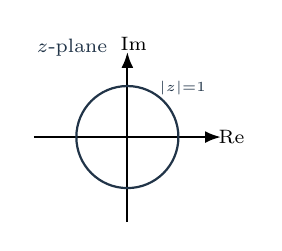
\begin{tikzpicture}[scale=0.54]
          % z-plane
          \begin{scope}[yshift=-3cm]
            \draw[-{Latex[length=2mm]}, thick] (-2.2,0) -- (2.2,0);
            \draw[-{Latex[length=2mm]}, thick] (0,-2.0) -- (0,2.0);
            \draw[thick, PrimaryColor] (0,0) circle (1.2);
            \node[PrimaryColor] at (1.3,1.15) {\tiny $|z|{=}1$};z
            \node[PrimaryColor] at (-1.3,2.1) {\scriptsize $z$-plane};
            \node at (0.15,2.2) {\scriptsize Im};
            \node at (2.45,0) {\scriptsize Re};
          \end{scope}
        \end{tikzpicture}
      \end{center}
    \end{column}
  \end{columns}
\end{frame}

\begin{frame}[t]{Why $z$ instead of $e^{s}$?}
  \small
  \begin{columns}[T]
    \begin{column}{0.54\textwidth}
      \begin{itemize}
        \item
          In DTFT, we set $T=1$ and work with $e^{j\omega n}$.
          We \emph{could} generalize the same way and write $e^{sn}$, $s = \sigma + j\omega$.
        \item      \textbf{But the map $s\mapsto e^{sT} = e^{\sigma T}\, e^{j\omega T}$ is many-to-one:} \\
          shifting $\omega$ by $\frac{2\pi}{T}$ gives the same $z = e^{sT}$. \\
          \vspace{0.1cm}

        \item
          In continuous time, $e^{j(\omega+2\pi/T)t}\neq e^{j\omega t}$ for general $t$, so distinct $s$ values still give distinct signals.
        \item
          In discrete time,
          $n$ is an \textbf{integer}, so $e^{j(\omega+2\pi/T)Tn} = e^{j\omega T n}$---different $s$ values produce the \emph{same} discrete-time signal.
        \item Using $z$ as a parameter solves this redundancy.

      \end{itemize}

      \begin{insightbox}{$z$ Parameterization}
        Parameterizing by $z$ collapses the redundancy in the $s$-plane. Also,
        as we will see, using $z$ makes the algebra and geometry of the transform much more intuitive.
      \end{insightbox}
    \end{column}
    \begin{column}{0.44\textwidth}
      \begin{center}
        \textbf{Many-to-one mapping}\\[0.15cm]

        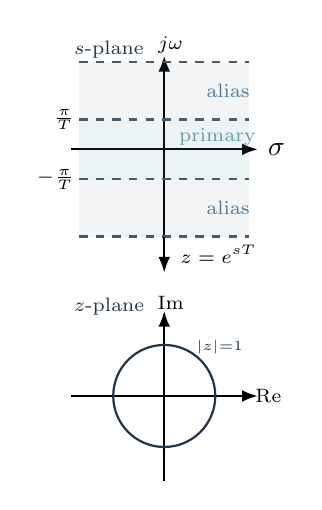
\begin{tikzpicture}[scale=0.54]
          % s-plane with strips
          \begin{scope}[yshift=2.8cm]
            \draw[-{Latex[length=2mm]}, thick] (-2.2,0) -- (2.2,0) node[right] {$\sigma$};
            \draw[-{Latex[length=2mm]}, thick] (0,-2.2) -- (0,2.2);
            \node at (0.15,2.45) {\scriptsize $j\omega$};
            \node[PrimaryColor] at (-1.3,2.35) {\scriptsize $s$-plane};
            % strips
            \fill[AccentColor, fill opacity=0.12] (-2.0,-0.7) rectangle (2.0,0.7);
            \draw[dashed, thick, DarkGray] (-2.0,0.7) -- (2.0,0.7);
            \draw[dashed, thick, DarkGray] (-2.0,-0.7) -- (2.0,-0.7);
            \fill[SecondaryColor, fill opacity=0.08] (-2.0,0.7) rectangle (2.0,2.05);
            \fill[SecondaryColor, fill opacity=0.08] (-2.0,-0.7) rectangle (2.0,-2.05);
            \draw[dashed, thick, DarkGray] (-2.0,2.05) -- (2.0,2.05);
            \draw[dashed, thick, DarkGray] (-2.0,-2.05) -- (2.0,-2.05);
            \node[AccentColor] at (1.25,0.3) {\scriptsize primary};
            \node[SecondaryColor] at (1.5,1.38) {\scriptsize alias};
            \node[SecondaryColor] at (1.5,-1.38) {\scriptsize alias};
            \node at (-2.35,0.7) {\scriptsize $\frac{\pi}{T}$};
            \node at (-2.55,-0.7) {\scriptsize $-\frac{\pi}{T}$};
          \end{scope}

          \draw[-{Latex[length=2mm]}, thick] (0,0.75) -- (0,-0.1);
          \node[right] at (0.15,0.33) {\scriptsize $z=e^{sT}$};

          % z-plane
          \begin{scope}[yshift=-3cm]
            \draw[-{Latex[length=2mm]}, thick] (-2.2,0) -- (2.2,0);
            \draw[-{Latex[length=2mm]}, thick] (0,-2.0) -- (0,2.0);
            \draw[thick, PrimaryColor] (0,0) circle (1.2);
            \node[PrimaryColor] at (1.3,1.15) {\tiny $|z|{=}1$};z
            \node[PrimaryColor] at (-1.3,2.1) {\scriptsize $z$-plane};
            \node at (0.15,2.2) {\scriptsize Im};
            \node at (2.45,0) {\scriptsize Re};
          \end{scope}
        \end{tikzpicture}
      \end{center}
    \end{column}
  \end{columns}
\end{frame}

\begin{frame}[t]{How the Mapping \texorpdfstring{$z=e^{sT}$}{z=e^(sT)} Changes the Geometry}
  \small
  \begin{columns}[T]
    \begin{column}{0.56\textwidth}
      The mapping $z=e^{sT}$ transforms $s$-plane geometry into $z$-plane geometry:

      \vspace{0.15cm}
      {\footnotesize
        \renewcommand{\arraystretch}{1.4}
        \begin{tabular}{@{}l@{\;$\;\longrightarrow\;$\;}l@{}}
          \toprule
          \textbf{$s$-plane} & \textbf{$z$-plane} \\
          \midrule
          Vertical line $\text{Re}\{s\}=\sigma_0$ & Circle $|z|=e^{\sigma_0 T}$ \\
          $j\omega$-axis ($\sigma_0=0$) & Unit circle $|z|=1$ \\
          ROC strip & ROC annulus \\
          \bottomrule
        \end{tabular}
      }

      \vspace{0.15cm}
      \begin{insightbox}{Consequence}
        \footnotesize
        The unit circle plays the same role in the $z$-plane that the $j\omega$-axis plays in the $s$-plane. ROC questions become questions about \textbf{radii}, not real parts.
      \end{insightbox}
    \end{column}
    \begin{column}{0.44\textwidth}
      \begin{center}
        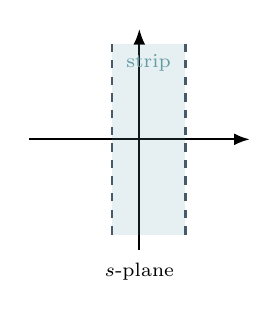
\begin{tikzpicture}[scale=0.78]
          \begin{scope}[xshift=0cm]
            \draw[-{Latex[length=2mm]}, thick] (-1.8,0) -- (1.8,0);
            \draw[-{Latex[length=2mm]}, thick] (0,-1.8) -- (0,1.8);
            \fill[AccentColor, fill opacity=0.16] (-0.45,-1.55) rectangle (0.75,1.55);
            \draw[dashed, thick, DarkGray] (-0.45,-1.55) -- (-0.45,1.55);
            \draw[dashed, thick, DarkGray] (0.75,-1.55) -- (0.75,1.55);
            \node[AccentColor] at (0.15,1.25) {\scriptsize strip};
            \node at (0,-2.15) {\scriptsize $s$-plane};
          \end{scope}
        \end{tikzpicture}

        \[
          z=e^{sT}
        \]

        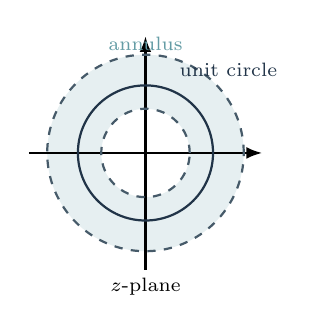
\begin{tikzpicture}[scale=0.78]
          \fill[AccentColor, fill opacity=0.16, even odd rule] (0,0) circle (1.6) (0,0) circle (0.72);
          \draw[-{Latex[length=2mm]}, thick] (-1.9,0) -- (1.9,0);
          \draw[-{Latex[length=2mm]}, thick] (0,-1.9) -- (0,1.9);
          \draw[dashed, thick, DarkGray] (0,0) circle (0.72);
          \draw[dashed, thick, DarkGray] (0,0) circle (1.6);
          \draw[thick, PrimaryColor] (0,0) circle (1.1);
          \node[AccentColor] at (0,1.78) {\scriptsize annulus};
          \node[PrimaryColor] at (1.35,1.35) {\scriptsize unit circle};
          \node at (0,-2.18) {\scriptsize $z$-plane};
        \end{tikzpicture}
      \end{center}
    \end{column}
  \end{columns}
\end{frame}

\begin{frame}[t]{The System Function \texorpdfstring{$H(z)$}{H(z)}}
  \small
  Since $z^n$ is an eigenfunction of DT-LTI systems, the system is completely characterized by its \textbf{system function}:
  \begin{conceptbox}{System Function}
    \vspace{-0.2cm}
    \[
      H(z) = \sum_{k=-\infty}^{\infty} h[k]\,z^{-k}
      \qquad\qquad
      x[n] = z^n \;\Longrightarrow\; y[n] = H(z)\,z^n
    \]
    \vspace{-0.2cm}
  \end{conceptbox}

  \vspace{0.15cm}
  \begin{columns}[T]
    \begin{column}{0.48\textwidth}
      \begin{insightbox}{What $H(z)$ Encodes}
        \footnotesize
      \begin{itemize}\setlength\itemsep{0pt}
          \item Convolution in time $\longrightarrow$ multiplication in $z$
            \[ Y(z) = H(z)\,X(z) \]
          \item Poles of $H(z)$ $\longrightarrow$ natural modes of the system
          \item Zeros of $H(z)$ $\longrightarrow$ frequencies the system blocks
        \end{itemize}
      \end{insightbox}
    \end{column}
    \begin{column}{0.48\textwidth}
      \begin{insightbox}{Parallel with Laplace}
        \footnotesize
        \renewcommand{\arraystretch}{1.3}
        \begin{tabular}{@{}l@{\quad}l@{}}
          Laplace & z-transform \\
          \midrule
          $H(s)$ & $H(z)$ \\
          $Y(s)=H(s)X(s)$ & $Y(z)=H(z)X(z)$ \\
          poles in LHP & poles inside UC \\
        \end{tabular}
      \end{insightbox}
    \end{column}
  \end{columns}
\end{frame}

\begin{frame}{Definition of the z-Transform and Its DTFT Connection}
  \small
  \begin{columns}[T]
    \begin{column}{0.58\textwidth}
      \begin{conceptbox}{z-Transform}
        \[
          X(z) \triangleq \sum_{n=-\infty}^{\infty} x[n]z^{-n}
        \]
      \end{conceptbox}

      \vspace{0.08cm}
      Write
      \[
        z = re^{j\omega}.
      \]
      Then
      \begin{align*}
        X(re^{j\omega})
        &= \sum_{n=-\infty}^{\infty} x[n](re^{j\omega})^{-n} \\
        &= \sum_{n=-\infty}^{\infty} \big(x[n]r^{-n}\big)e^{-j\omega n}.
      \end{align*}
      Hence
      \[
        X(re^{j\omega}) = \mathcal{F}\{x[n]r^{-n}\}.
      \]

      \vspace{0.08cm}
      Setting $r=1$ restricts the z-transform to the unit circle, so we recover the DTFT. Therefore the DTFT exists iff the ROC includes $|z|=1$.
    \end{column}
    \begin{column}{0.42\textwidth}
      \begin{center}
        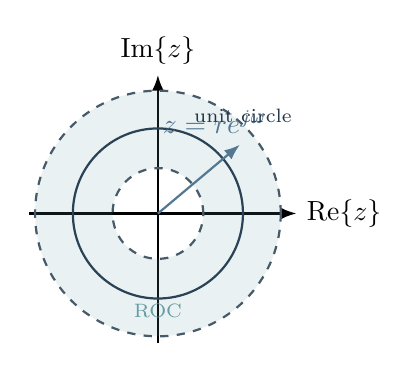
\begin{tikzpicture}[scale=0.8]
          \draw[-{Latex[length=2mm]}, thick] (-2.05,0) -- (2.2,0) node[right] {$\text{Re}\{z\}$};
          \draw[-{Latex[length=2mm]}, thick] (0,-2.05) -- (0,2.2) node[above] {$\text{Im}\{z\}$};
          \draw[thick, PrimaryColor] (0,0) circle (1.35);
          \fill[AccentColor, fill opacity=0.14, even odd rule] (0,0) circle (1.95) (0,0) circle (0.72);
          \draw[dashed, thick, DarkGray] (0,0) circle (0.72);
          \draw[dashed, thick, DarkGray] (0,0) circle (1.95);
          \draw[-{Latex[length=2mm]}, thick, SecondaryColor] (0,0) -- (40:1.7);
          \node[SecondaryColor] at (0.9,1.45) {$z=re^{j\omega}$};
          \node[PrimaryColor] at (1.35,1.55) {\scriptsize unit circle};
          \node[AccentColor] at (0,-1.55) {\scriptsize ROC};
        \end{tikzpicture}

        \vspace{0.1cm}
        \begin{insightbox}{Fourier and z}
          The DTFT is the restriction of the z-transform to $|z|=1$.
        \end{insightbox}
      \end{center}
    \end{column}
  \end{columns}
\end{frame}

\section{Examples and the ROC}

\begin{frame}[t]{Example 10.1: A Right-Sided Exponential}
  \small
  \begin{columns}[T]
    \begin{column}{0.53\textwidth}
      Consider
      \[
        x[n]=a^n u[n].
      \]
      Then
      \begin{align*}
        X(z)
        &= \sum_{n=0}^{\infty} a^n z^{-n}
        = \sum_{n=0}^{\infty} (az^{-1})^n \\
        &= \frac{1}{1-az^{-1}}
        = \frac{z}{z-a},
        \qquad |z|>|a|.
      \end{align*}

      \begin{itemize}
        \item This is the discrete-time analogue of $e^{-at}u(t)$ in the Laplace chapter.
        \item Pole at $z=a$, zero at $z=0$.
        \item The ROC is the exterior of a circle.
        \item If $|a|<1$, the ROC includes the unit circle, so the DTFT exists.
      \end{itemize}
    \end{column}
    \begin{column}{0.47\textwidth}
      \textbf{Sequence for $a=0.6$}\\[-0.05cm]
      \begin{center}
        \begin{tikzpicture}
          \begin{axis}[
              width=0.95\textwidth, height=3.4cm,
              axis lines=middle, axis line style={-{Latex[length=2mm]}},
              xmin=-1.2, xmax=7.4, ymin=-0.1, ymax=1.15,
              xtick={0,1,2,3,4,5,6}, ytick={1},
              yticklabels={$1$},
              xlabel={$n$}, ylabel={$x[n]$},
              xlabel style={anchor=west, at={(axis cs:7.55,0)}},
              ylabel style={anchor=south, at={(axis cs:0,1.2)}},
              clip=false
            ]
            \addplot+[discrete, samples at={0,1,2,3,4,5,6}] {0.6^x};
          \end{axis}
        \end{tikzpicture}
      \end{center}

      \textbf{Pole-zero plot and ROC}\\[-0.05cm]
      \begin{center}
        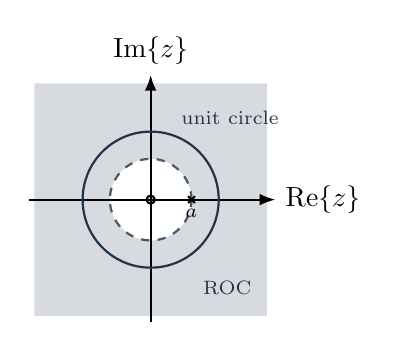
\begin{tikzpicture}[scale=0.72]
          \fill[PrimaryColor, fill opacity=0.18, even odd rule] (-2.05,-2.05) rectangle (2.05,2.05) (0,0) circle (0.72);
          \draw[-{Latex[length=2mm]}, thick] (-2.15,0) -- (2.2,0) node[right] {$\text{Re}\{z\}$};
          \draw[-{Latex[length=2mm]}, thick] (0,-2.15) -- (0,2.2) node[above] {$\text{Im}\{z\}$};
          \draw[thick, PrimaryColor] (0,0) circle (1.2);
          \draw[dashed, thick, DarkGray] (0,0) circle (0.72);
          \draw[thick] (0.66,0.06) -- (0.78,-0.06);
          \draw[thick] (0.66,-0.06) -- (0.78,0.06);
          \draw[thick] (0,0) circle (0.07);
          \node[PrimaryColor] at (1.4,1.45) {\scriptsize unit circle};
          \node[PrimaryColor] at (1.35,-1.55) {\scriptsize ROC};
          \node at (0.72,-0.25) {\scriptsize $a$};
        \end{tikzpicture}
      \end{center}
    \end{column}
  \end{columns}
\end{frame}

\begin{frame}[t]{Example 10.2: A Left-Sided Exponential}
  \footnotesize
  \begin{columns}[T]
    \begin{column}{0.53\textwidth}
      Consider
      \[
        x[n] = -a^n u[-n-1].
      \]
      Then
      \begin{align*}
        X(z)
        &= \sum_{n=-\infty}^{-1} -a^n z^{-n} \\
        &= -\sum_{m=1}^{\infty} a^{-m} z^m
        = -\sum_{m=1}^{\infty} (a^{-1}z)^m \\
        &= \frac{1}{1-az^{-1}}
        = \frac{z}{z-a},
        \qquad |z|<|a|.
      \end{align*}

      \begin{itemize}
        \item Same algebraic expression as Example 10.1.
        \item But now the ROC is the interior of the circle.
        \item This is exactly the same message we saw with Laplace transforms:
          algebraic form alone is not enough.
      \end{itemize}
    \end{column}
    \begin{column}{0.47\textwidth}
      \textbf{Sequence for $a=0.6$}\\[-0.05cm]
      \begin{center}
        \begin{tikzpicture}
          \begin{axis}[
              width=0.92\textwidth, height=2.85cm,
              axis lines=middle, axis line style={-{Latex[length=2mm]}},
              xmin=-6.3, xmax=1.1, ymin=-5.2, ymax=0.3,
              xtick={-5,-4,-3,-2,-1}, ytick={-1},
              yticklabels={$-1$},
              xlabel={$n$}, ylabel={$x[n]$},
              xlabel style={anchor=west, at={(axis cs:1.25,0)}},
              ylabel style={anchor=south, at={(axis cs:0,0.35)}},
              clip=false
            ]
            \addplot+[discrete, samples at={-5,-4,-3,-2,-1}] {-0.6^x};
          \end{axis}
        \end{tikzpicture}
      \end{center}

      \textbf{Pole-zero plot and ROC}\\[-0.05cm]
      \begin{center}
        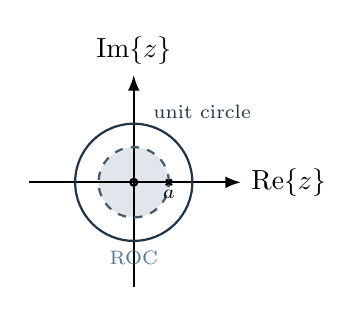
\begin{tikzpicture}[scale=0.62]
          \fill[SecondaryColor, fill opacity=0.18] (0,0) circle (0.72);
          \draw[-{Latex[length=2mm]}, thick] (-2.15,0) -- (2.2,0) node[right] {$\text{Re}\{z\}$};
          \draw[-{Latex[length=2mm]}, thick] (0,-2.15) -- (0,2.2) node[above] {$\text{Im}\{z\}$};
          \draw[thick, PrimaryColor] (0,0) circle (1.2);
          \draw[dashed, thick, DarkGray] (0,0) circle (0.72);
          \draw[thick] (0.66,0.06) -- (0.78,-0.06);
          \draw[thick] (0.66,-0.06) -- (0.78,0.06);
          \draw[thick] (0,0) circle (0.07);
          \node[PrimaryColor] at (1.4,1.45) {\scriptsize unit circle};
          \node[SecondaryColor] at (0,-1.55) {\scriptsize ROC};
          \node at (0.72,-0.25) {\scriptsize $a$};
        \end{tikzpicture}
      \end{center}
    \end{column}
  \end{columns}
\end{frame}

\begin{frame}[t]{Why the ROC Matters}
  \footnotesize
  \begin{columns}[T]
    \begin{column}{0.56\textwidth}
      \begin{itemize}
        \item Examples 10.1 and 10.2 have the same
          \[
            X(z)=\frac{z}{z-a},
          \]
          but they are different sequences because the ROCs differ.
        \item So a z-transform is specified by
          \[
            \text{algebraic expression} + \text{ROC}.
          \]
        \item For rational transforms:
          \begin{itemize}
            \item \textbf{zeros} are the roots of the numerator,
            \item \textbf{poles} are the roots of the denominator.
          \end{itemize}
        \item The ROC tells us:
          \begin{itemize}
            \item whether the sequence is right-sided, left-sided, or two-sided,
            \item whether the DTFT exists,
            \item and later, whether an LTI system is causal or stable.
          \end{itemize}
      \end{itemize}
      \[
        \text{Laplace: half-planes or strips}
        \qquad \Longleftrightarrow \qquad
        \text{z-transform: disks, exteriors, annuli}
      \]
    \end{column}
    \begin{column}{0.44\textwidth}
      \begin{center}
        \textbf{Same poles and zeros, different ROC}\\[0.05cm]
        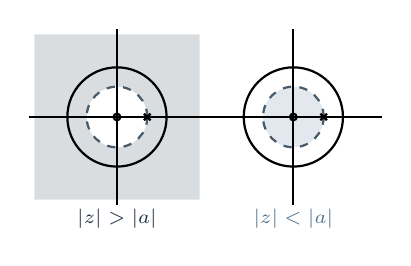
\begin{tikzpicture}[scale=0.7]
          \begin{scope}[xshift=-1.6cm]
            \fill[PrimaryColor, fill opacity=0.17, even odd rule] (-1.5,-1.5) rectangle (1.5,1.5) (0,0) circle (0.55);
            \draw[thick] (0,0) circle (0.9);
            \draw[dashed, thick, DarkGray] (0,0) circle (0.55);
            \draw[thick] (-1.6,0) -- (1.6,0);
            \draw[thick] (0,-1.6) -- (0,1.6);
            \draw[thick] (0.49,0.06) -- (0.61,-0.06);
            \draw[thick] (0.49,-0.06) -- (0.61,0.06);
            \draw[thick] (0,0) circle (0.06);
            \node[PrimaryColor] at (0,-1.85) {\scriptsize $|z|>|a|$};
          \end{scope}
          \begin{scope}[xshift=1.6cm]
            \fill[SecondaryColor, fill opacity=0.17] (0,0) circle (0.55);
            \draw[thick] (0,0) circle (0.9);
            \draw[dashed, thick, DarkGray] (0,0) circle (0.55);
            \draw[thick] (-1.6,0) -- (1.6,0);
            \draw[thick] (0,-1.6) -- (0,1.6);
            \draw[thick] (0.49,0.06) -- (0.61,-0.06);
            \draw[thick] (0.49,-0.06) -- (0.61,0.06);
            \draw[thick] (0,0) circle (0.06);
            \node[SecondaryColor] at (0,-1.85) {\scriptsize $|z|<|a|$};
          \end{scope}
        \end{tikzpicture}
      \end{center}
    \end{column}
  \end{columns}
\end{frame}

\begin{frame}[t]{Example 10.3: Sum of Two Exponentials}
  \small
  \begin{columns}[T]
    \begin{column}{0.58\textwidth}
      \[
        x[n] = 7\left(\frac{1}{3}\right)^n u[n] - 6\left(\frac{1}{2}\right)^n u[n].
      \]
      By linearity and Example 10.1,
      \begin{align*}
        X(z)
        &= \frac{7}{1-\frac{1}{3}z^{-1}} - \frac{6}{1-\frac{1}{2}z^{-1}} \\
        &= \frac{1-\frac{3}{2}z^{-1}}{\left(1-\frac{1}{3}z^{-1}\right)\left(1-\frac{1}{2}z^{-1}\right)} \\
        &= \frac{z\left(z-\frac{2}{3}\right)}{\left(z-\frac{1}{3}\right)\left(z-\frac{1}{2}\right)}.
      \end{align*}
      Since both components are right-sided,
      \[
        \text{ROC}: |z|>\frac{1}{2}.
      \]

      \begin{itemize}
        \item Poles at $z=\frac{1}{3},\frac{1}{2}$.
        \item Zeros at $z=0,\frac{2}{3}$.
        \item The ROC is outside the outermost pole, exactly as in the Laplace chapter.
      \end{itemize}
    \end{column}
    \begin{column}{0.42\textwidth}
      \begin{center}
        \textbf{Pole-zero plot}\\[0.08cm]
        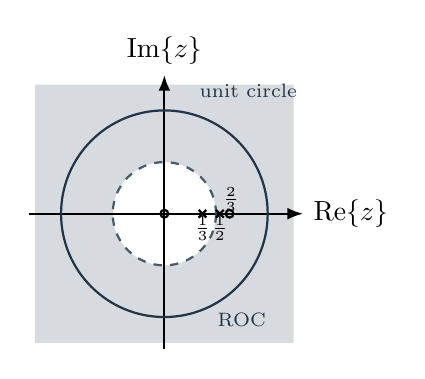
\begin{tikzpicture}[scale=0.82]
          \fill[PrimaryColor, fill opacity=0.18, even odd rule] (-2,-2) rectangle (2,2) (0,0) circle (0.8);
          \draw[-{Latex[length=2mm]}, thick] (-2.1,0) -- (2.15,0) node[right] {$\text{Re}\{z\}$};
          \draw[-{Latex[length=2mm]}, thick] (0,-2.1) -- (0,2.15) node[above] {$\text{Im}\{z\}$};
          \draw[thick, PrimaryColor] (0,0) circle (1.6);
          \draw[dashed, thick, DarkGray] (0,0) circle (0.8);
          \draw[thick] (0.53,0.06) -- (0.65,-0.06);
          \draw[thick] (0.53,-0.06) -- (0.65,0.06);
          \draw[thick] (0.8,0.06) -- (0.92,-0.06);
          \draw[thick] (0.8,-0.06) -- (0.92,0.06);
          \draw[thick] (0,0) circle (0.06);
          \draw[thick] (1.01,0) circle (0.06);
          \node at (0.59,-0.23) {\scriptsize $\frac13$};
          \node at (0.86,-0.23) {\scriptsize $\frac12$};
          \node at (1.03,0.22) {\scriptsize $\frac23$};
          \node[PrimaryColor] at (1.3,1.9) {\scriptsize unit circle};
          \node[PrimaryColor] at (1.2,-1.65) {\scriptsize ROC};
        \end{tikzpicture}
      \end{center}
    \end{column}
  \end{columns}
\end{frame}

\begin{frame}[t]{Example 10.4: A Damped Sinusoid}
  \small
  \begin{columns}[T]
    \begin{column}{0.58\textwidth}
      Consider
      \[
        x[n]=\left(\frac{1}{3}\right)^n \sin\left(\frac{\pi}{4}n\right)u[n].
      \]
      Use Euler's identity:
      \[
        \sin\left(\frac{\pi}{4}n\right)
        = \frac{e^{j\pi n/4}-e^{-j\pi n/4}}{2j}.
      \]
      Then
      \begin{align*}
        X(z)
        &= \frac{1}{2j}\frac{1}{1-\frac13 e^{j\pi/4}z^{-1}}
        - \frac{1}{2j}\frac{1}{1-\frac13 e^{-j\pi/4}z^{-1}} \\
        &= \frac{\frac{\sqrt{2}}{3}z^{-1}}
        {1-\frac{\sqrt{2}}{3}z^{-1}+\frac{1}{9}z^{-2}} \\
        &= \frac{\frac{\sqrt{2}}{3}z}{\left(z-\frac13 e^{j\pi/4}\right)\left(z-\frac13 e^{-j\pi/4}\right)}.
      \end{align*}
      Both exponential components are right-sided, so
      \[
        \text{ROC}: |z|>\frac13.
      \]
    \end{column}
    \begin{column}{0.42\textwidth}
      \textbf{Sequence and ROC}\\[-0.05cm]
      \begin{center}
        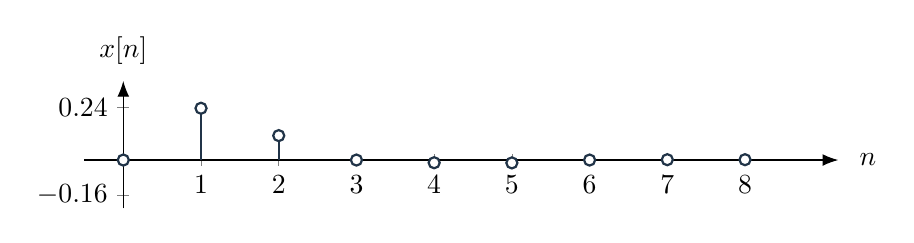
\begin{tikzpicture}
          \begin{axis}[
              width=0.92\textwidth, height=3.2cm,
              axis lines=middle, axis line style={-{Latex[length=2mm]}},
              xmin=-0.5, xmax=9.2, ymin=-0.22, ymax=0.36,
              xtick={0,1,2,3,4,5,6,7,8},
              ytick={0.24,-0.16},
              xlabel={$n$}, ylabel={$x[n]$},
              xlabel style={anchor=west, at={(axis cs:9.35,0)}},
              ylabel style={anchor=south, at={(axis cs:0,0.39)}},
              clip=false
            ]
            \addplot+[discrete] coordinates {
              (0,0) (1,0.2357) (2,0.1111) (3,0) (4,-0.0123)
              (5,-0.0131) (6,0) (7,0.0015) (8,0.00152)
            };
          \end{axis}
        \end{tikzpicture}

        \vspace{0.15cm}
        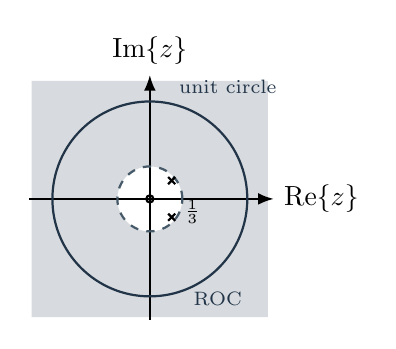
\begin{tikzpicture}[scale=0.75]
          \fill[PrimaryColor, fill opacity=0.18, even odd rule] (-2,-2) rectangle (2,2) (0,0) circle (0.55);
          \draw[-{Latex[length=2mm]}, thick] (-2.05,0) -- (2.1,0) node[right] {$\text{Re}\{z\}$};
          \draw[-{Latex[length=2mm]}, thick] (0,-2.05) -- (0,2.1) node[above] {$\text{Im}\{z\}$};
          \draw[thick, PrimaryColor] (0,0) circle (1.65);
          \draw[dashed, thick, DarkGray] (0,0) circle (0.55);
          \draw[thick] (0.31,0.37) -- (0.43,0.25);
          \draw[thick] (0.31,0.25) -- (0.43,0.37);
          \draw[thick] (0.31,-0.37) -- (0.43,-0.25);
          \draw[thick] (0.31,-0.25) -- (0.43,-0.37);
          \draw[thick] (0,0) circle (0.06);
          \node at (0.72,-0.22) {\scriptsize $\frac13$};
          \node[PrimaryColor] at (1.32,1.9) {\scriptsize unit circle};
          \node[PrimaryColor] at (1.15,-1.7) {\scriptsize ROC};
        \end{tikzpicture}
      \end{center}
    \end{column}
  \end{columns}
\end{frame}

\begin{frame}[t]{ROC Properties 1--2}
  \footnotesize
  \begin{conceptbox}{Property 1}
    The ROC of $X(z)$ is a \textbf{ring centered at the origin}
  \end{conceptbox}
  \vspace{0.1cm}
  \[
    X(re^{j\omega})
    =
    \sum_{n=-\infty}^{\infty}x[n]r^{-n}e^{-j\omega n},
    \qquad
    \sum_{n=-\infty}^{\infty}|x[n]|r^{-n}<\infty.
  \]
  Absolute convergence depends on the radius $r=|z|$, not on the angle.

  \vspace{0.3cm}
  \begin{conceptbox}{Property 2}
    The ROC cannot contain any poles.
  \end{conceptbox}
  At a pole, $X(z)$ is unbounded. Zeros may lie in the ROC; poles may only lie on its boundary or outside it.

\end{frame}

\begin{frame}[t]{ROC Property 3: Finite-Duration Sequences}
  \small
  \begin{conceptbox}{Property 3}
    If $x[n]$ is finite-duration, the ROC is the entire z-plane, except possibly at $z=0$ and/or $z=\infty$.
  \end{conceptbox}
  \vspace{0.04cm}

  \textit{Justification:} Only finitely many terms appear:
  \[
    X(z)=\sum_{n=N_1}^{N_2}x[n]z^{-n}.
  \]
  Thus every \textbf{finite, nonzero} $z$ is safe.

  But note there are two special cases:
  \begin{itemize}
    \item A sample at $n>0$ creates negative powers of $z$ and can exclude $z=0$. \\
      Since as $|z|\to 0$, $z^{-n}\to\infty$ for $n>0$.
    \item A sample at $n<0$ creates positive powers of $z$ and can exclude $z=\infty$. \\
      Since as $|z|\to\infty$, $z^{-n}\to\infty$ for $n<0$.
  \end{itemize}
  As a result, if $N_1\ge 0$, the ROC includes $\infty$; if $N_2\le 0$, it includes $0$.
\end{frame}

\begin{frame}[t]{Example 10.5: Finite-Duration Sequences}
  \small
  \begin{columns}[T]
    \begin{column}{0.56\textwidth}
      \vspace{0.5cm}
      \textbf{Impulse}
      \[
        \delta[n]
        \stackrel{\mathcal{Z}}{\longleftrightarrow}
        \sum_{n=-\infty}^{\infty}\delta[n]z^{-n} = 1.
      \]
      ROC: entire z-plane, including $0$ and $\infty$.

      \vspace{0.4cm}
      \textbf{Delayed impulse}
      \[
        \delta[n-1]
        \stackrel{\mathcal{Z}}{\longleftrightarrow}
        \sum_{n=-\infty}^{\infty}\delta[n-1]z^{-n} = z^{-1}.
      \]
      ROC: entire z-plane except $z=0$.

      \vspace{0.4cm}
      \textbf{Advanced impulse}
      \[
        \delta[n+1]
        \stackrel{\mathcal{Z}}{\longleftrightarrow}
        z
      \]
      ROC: entire finite z-plane, but not $z=\infty$.

      \vspace{0.5cm}
      These examples show how positive powers of $z$ threaten $\infty$
      and negative powers threaten $0$.
    \end{column}
    \begin{column}{0.44\textwidth}
      \begin{center}
        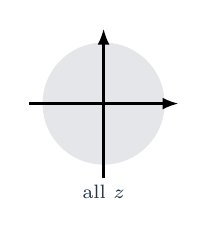
\begin{tikzpicture}[scale=0.5]
          \fill[PrimaryColor, fill opacity=0.12] (0,0) circle (1.55);
          \draw[-{Latex[length=2mm]}, thick] (-1.9,0) -- (1.9,0);
          \draw[-{Latex[length=2mm]}, thick] (0,-1.9) -- (0,1.9);
          \node[PrimaryColor] at (0,-2.25) {\scriptsize all $z$};
        \end{tikzpicture}

        \vspace{0.12cm}
        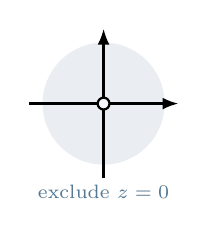
\begin{tikzpicture}[scale=0.5]
          \fill[SecondaryColor, fill opacity=0.12, even odd rule] (0,0) circle (1.55) (0,0) circle (0.15);
          \draw[-{Latex[length=2mm]}, thick] (-1.9,0) -- (1.9,0);
          \draw[-{Latex[length=2mm]}, thick] (0,-1.9) -- (0,1.9);
          \fill[BackgroundColor] (0,0) circle (0.15);
          \draw[thick] (0,0) circle (0.15);
          \node[SecondaryColor] at (0,-2.25) {\scriptsize exclude $z=0$};
        \end{tikzpicture}

        \vspace{0.12cm}
        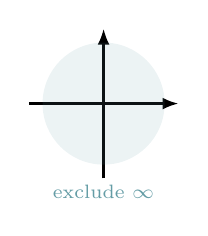
\begin{tikzpicture}[scale=0.5]
          \draw[-{Latex[length=2mm]}, thick] (-1.9,0) -- (1.9,0);
          \draw[-{Latex[length=2mm]}, thick] (0,-1.9) -- (0,1.9);
          \fill[AccentColor, fill opacity=0.12] (0,0) circle (1.55);
          \node[AccentColor] at (0,-2.25) {\scriptsize exclude $\infty$};
        \end{tikzpicture}
      \end{center}
    \end{column}
  \end{columns}
\end{frame}

\begin{frame}[t]{ROC Property 4: Right-Sided Sequences}
  \small
  \begin{conceptbox}{Property 4}
    If $x[n]$ is a right-sided sequence, and if the circle $|z|=r_0$ is in the ROC,
    then all finite values of $z$ for which $|z|>r_0$ will also be in the ROC.
  \end{conceptbox}

  \vspace{0.4cm}
  \begin{columns}[T]
    \begin{column}{0.50\textwidth}
      \footnotesize
      Right-sided means $x[n]=0$ for $n<N_1$, so
      \[
        X(z)=\sum_{n=N_1}^{\infty}x[n]z^{-n},
        \quad
        \sum_{n=N_1}^{\infty}|x[n]|r_0^{-n}<\infty
      \]
      when $|z|=r_0$ lies in the ROC. For any $r_1>r_0$:
      \[
        |x[n]|r_1^{-n}
        = |x[n]|r_0^{-n}\!\left(\tfrac{r_0}{r_1}\right)^{\!n}.
      \]
      Since $0 < r_0/r_1<1$, the extra factor decays with $n$ $\Rightarrow$ absolute summability at $r_1$ is guaranteed.

      \vspace{0.15cm}
      \textbf{Endpoint nuance:}
      if $N_1<0$, $\infty$ may be excluded; for causal sequences ($N_1\ge 0$), $\infty\in$ ROC.
    \end{column}
    \begin{column}{0.46\textwidth}
      \begin{center}
        \textbf{Faster decay for $r_1>r_0$}\\[0.15cm]
        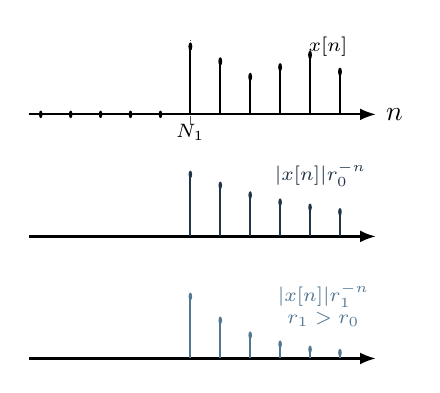
\begin{tikzpicture}[x=0.38cm,y=0.82cm]
          \begin{scope}[yshift=3.1cm]
            \draw[-{Latex[length=2mm]}, thick] (-5.4,0) -- (6.2,0) node[right] {$n$};
            \foreach \x in {-5,-4,-3,-2,-1}
            \fill (\x,0) circle (0.06);
            \draw[dashed, DarkGray] (0,-0.15) -- (0,1.15);
            \node[below] at (0,0) {\scriptsize $N_1$};
            \foreach \x/\h in {0/1.05,1/0.82,2/0.58,3/0.73,4/0.92,5/0.66}
            {
              \draw[thick] (\x,0)--(\x,\h);
              \fill (\x,\h) circle (0.065);
            }
            \node at (4.6,1.05) {\scriptsize $x[n]$};
          \end{scope}

          \begin{scope}[yshift=1.55cm]
            \draw[-{Latex[length=2mm]}, thick] (-5.4,0) -- (6.2,0);
            \foreach \x/\h in {0/0.96,1/0.79,2/0.64,3/0.53,4/0.45,5/0.38}
            {
              \draw[thick, PrimaryColor] (\x,0)--(\x,\h);
              \fill[PrimaryColor] (\x,\h) circle (0.06);
            }
            \node[PrimaryColor] at (4.35,0.96) {\scriptsize $|x[n]|r_0^{-n}$};
          \end{scope}

          \begin{scope}
            \draw[-{Latex[length=2mm]}, thick] (-5.4,0) -- (6.2,0);
            \foreach \x/\h in {0/0.96,1/0.59,2/0.36,3/0.22,4/0.14,5/0.09}
            {
              \draw[thick, SecondaryColor] (\x,0)--(\x,\h);
              \fill[SecondaryColor] (\x,\h) circle (0.06);
            }
            \node[SecondaryColor] at (4.45,0.98) {\scriptsize $|x[n]|r_1^{-n}$};
            \node[SecondaryColor] at (4.45,0.6) {\scriptsize $r_1>r_0$};
          \end{scope}
        \end{tikzpicture}
      \end{center}
    \end{column}
  \end{columns}
\end{frame}

\begin{frame}[t]{ROC Property 5: Left-Sided Sequences}
  \small
  \begin{conceptbox}{Property 5}
    If $x[n]$ is a left-sided sequence, and if the circle $|z|=r_0$ is in the ROC,
    then all values of $z$ for which $0<|z|<r_0$ will also be in the ROC.
  \end{conceptbox}

  \vspace{0.4cm}
  \begin{columns}[T]
    \begin{column}{0.50\textwidth}
      \footnotesize
      Left-sided means $x[n]=0$ for $n>N_2$, so
      \[
        X(z)=\sum_{n=-\infty}^{N_2}x[n]z^{-n},
        \quad
        \sum_{n=-\infty}^{N_2}|x[n]|r_0^{-n}<\infty
      \]
      when $|z|=r_0$ lies in the ROC. For any $0<r_1<r_0$:
      \[
        |x[n]|r_1^{-n}
        = |x[n]|r_0^{-n}\!\left(\tfrac{r_0}{r_1}\right)^{\!n}.
      \]
      Since $r_0/r_1>1$ but $n\to -\infty$, the extra factor decays $\Rightarrow$ absolute summability at $r_1$ is guaranteed.

      \vspace{0.15cm}
      \textbf{Endpoint nuance:}
      if $N_2>0$, $0$ may be excluded; for anticausal sequences ($N_2\le 0$), $0\in$ ROC.
    \end{column}
    \begin{column}{0.46\textwidth}
      \begin{center}
        \textbf{Faster decay for $0<r_1<r_0$}\\[0.15cm]
        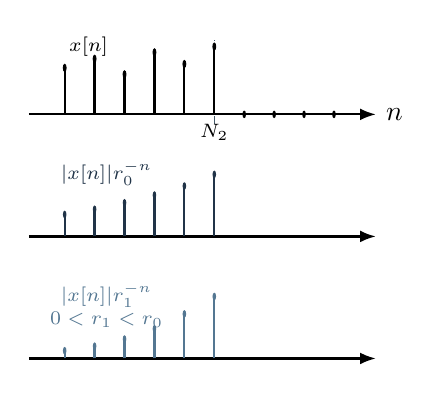
\begin{tikzpicture}[x=0.38cm,y=0.82cm]
          \begin{scope}[yshift=3.1cm]
            \draw[-{Latex[length=2mm]}, thick] (-6.2,0) -- (5.4,0) node[right] {$n$};
            \draw[dashed, DarkGray] (0,-0.15) -- (0,1.15);
            \node[below] at (0,0) {\scriptsize $N_2$};
            \foreach \x/\h in {-5/0.72,-4/0.86,-3/0.62,-2/0.96,-1/0.78,0/1.05}
            {
              \draw[thick] (\x,0)--(\x,\h);
              \fill (\x,\h) circle (0.065);
            }
            \foreach \x in {1,2,3,4,5}
            \fill (\x,0) circle (0.06);
            \node at (-4.2,1.05) {\scriptsize $x[n]$};
          \end{scope}

          \begin{scope}[yshift=1.55cm]
            \draw[-{Latex[length=2mm]}, thick] (-6.2,0) -- (5.4,0);
            \foreach \x/\h in {-5/0.34,-4/0.42,-3/0.52,-2/0.64,-1/0.78,0/0.96}
            {
              \draw[thick, PrimaryColor] (\x,0)--(\x,\h);
              \fill[PrimaryColor] (\x,\h) circle (0.06);
            }
            \node[PrimaryColor] at (-3.6,0.98) {\scriptsize $|x[n]|r_0^{-n}$};
          \end{scope}

          \begin{scope}
            \draw[-{Latex[length=2mm]}, thick] (-6.2,0) -- (5.4,0);
            \foreach \x/\h in {-5/0.12,-4/0.19,-3/0.30,-2/0.46,-1/0.69,0/0.96}
            {
              \draw[thick, SecondaryColor] (\x,0)--(\x,\h);
              \fill[SecondaryColor] (\x,\h) circle (0.06);
            }
            \node[SecondaryColor] at (-3.6,0.98) {\scriptsize $|x[n]|r_1^{-n}$};
            \node[SecondaryColor] at (-3.6,0.6) {\scriptsize $0<r_1<r_0$};
          \end{scope}
        \end{tikzpicture}
      \end{center}
    \end{column}
  \end{columns}
\end{frame}

\begin{frame}[t]{ROC Property 6: Two-Sided Sequences}
  \small
  \begin{columns}[T]
    \begin{column}{0.52\textwidth}
      \begin{conceptbox}{Property 6}
        If $x[n]$ is two-sided and has a z-transform, the ROC is an annulus.
      \end{conceptbox}

      Split a two-sided sequence into
      \[
        x[n]=x[n]u[n-N]+x[n]\bigl(1-u[n-N]\bigr).
      \]
      The right-sided part contributes an exterior ROC, and the left-sided part contributes an interior ROC.

      \begin{insightbox}{Overlap test}
        The z-transform exists only if those two ROCs overlap.
        When they do, the overlap is a ring: $r_1<|z|<r_2$.
      \end{insightbox}
    \end{column}
    \begin{column}{0.48\textwidth}
      \begin{center}
        \textbf{Exterior $\cap$ interior $=$ annulus}\\[0.06cm]
        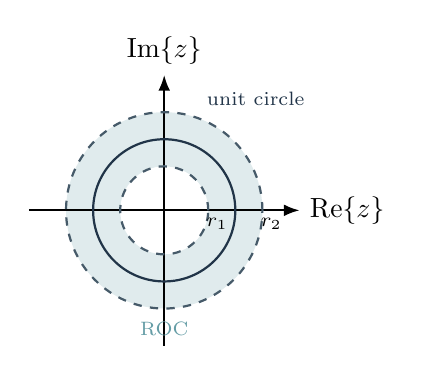
\begin{tikzpicture}[scale=0.86]
          \fill[AccentColor, fill opacity=0.2, even odd rule] (0,0) circle (1.45) (0,0) circle (0.65);
          \draw[-{Latex[length=2mm]}, thick] (-2.0,0) -- (2.0,0) node[right] {$\text{Re}\{z\}$};
          \draw[-{Latex[length=2mm]}, thick] (0,-2.0) -- (0,2.0) node[above] {$\text{Im}\{z\}$};
          \draw[dashed, thick, DarkGray] (0,0) circle (0.65);
          \draw[dashed, thick, DarkGray] (0,0) circle (1.45);
          \draw[thick, PrimaryColor] (0,0) circle (1.05);
          \node at (0.78,-0.2) {\scriptsize $r_1$};
          \node at (1.58,-0.2) {\scriptsize $r_2$};
          \node[PrimaryColor] at (1.35,1.65) {\scriptsize unit circle};
          \node[AccentColor] at (0,-1.75) {\scriptsize ROC};
        \end{tikzpicture}
      \end{center}
    \end{column}
  \end{columns}
\end{frame}

\begin{frame}[t]{Example 10.6: A Finite-Length Exponential}
  \small
  \begin{columns}[T]
    \begin{column}{0.56\textwidth}
      For
      \[
        x[n] =
        \begin{cases}
          a^n, & 0\le n\le N-1,\ a>0 \\
          0, & \text{otherwise}
        \end{cases}
      \]
      we have
      \begin{align*}
        X(z)
        &= \sum_{n=0}^{N-1} a^n z^{-n}
        = \frac{1-(az^{-1})^N}{1-az^{-1}} \\
        &= \frac{z\left[1-a^N z^{-N}\right]}{z-a}.
      \end{align*}
      Since the sequence is finite-duration, the ROC is all $z$ except possibly $z=0$.

      \vspace{0.08cm}
      After canceling the factor at $z=a$, the zeros are
      \[
        z_k = a e^{j2\pi k/N}, \qquad k=1,2,\dots,N-1,
      \]
      and there are $N-1$ poles at the origin.

      \vspace{0.08cm}
      This is a beautiful discrete-time picture:
      the zeros lie evenly on a circle of radius $a$.
    \end{column}
    \begin{column}{0.44\textwidth}
      \begin{center}
        \textbf{Pole-zero pattern for $N=8$}\\[0.08cm]
        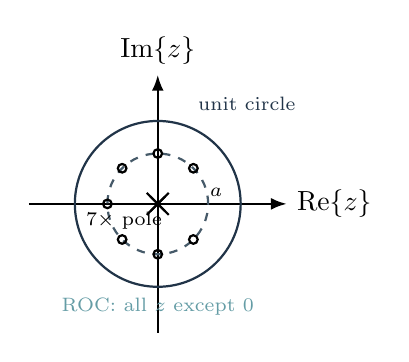
\begin{tikzpicture}[scale=0.78]
          \draw[-{Latex[length=2mm]}, thick] (-2.1,0) -- (2.1,0) node[right] {$\text{Re}\{z\}$};
          \draw[-{Latex[length=2mm]}, thick] (0,-2.1) -- (0,2.1) node[above] {$\text{Im}\{z\}$};
          \draw[thick, PrimaryColor] (0,0) circle (1.35);
          \draw[dashed, thick, DarkGray] (0,0) circle (0.82);
          \foreach \ang in {45,90,135,180,225,270,315}
          \draw[thick] ({0.82*cos(\ang)},{0.82*sin(\ang)}) circle (0.07);
          \draw[thick] (-0.18,-0.18) -- (0.18,0.18);
          \draw[thick] (-0.18,0.18) -- (0.18,-0.18);
          \draw[thick] (-0.12,-0.12) -- (0.12,0.12);
          \draw[thick] (-0.12,0.12) -- (0.12,-0.12);
          \node at (0.95,0.18) {\scriptsize $a$};
          \node at (-0.55,-0.28) {\scriptsize $7\times$ pole};
          \node[PrimaryColor] at (1.45,1.63) {\scriptsize unit circle};
          \node[AccentColor] at (0,-1.68) {\scriptsize ROC: all $z$ except $0$};
        \end{tikzpicture}
      \end{center}
    \end{column}
  \end{columns}
\end{frame}

\begin{frame}[t]{Example 10.7: \texorpdfstring{$b^{-|n|}$}{b^-|n|}}
  \small
  \begin{columns}[T]
    \begin{column}{0.56\textwidth}
      Let
      \[
        x[n]=b^{-|n|}, \qquad b>0.
      \]
      Write it as
      \[
        x[n]=b^{-n}u[n]+b^n u[-n-1].
      \]
      Then the ROC depends strongly on $b$:
      \begin{itemize}
        \item If $0<b<1$, the right-sided part needs $|z|>b$ and the left-sided part needs $|z|<1/b$.
          Hence
          \[
            b<|z|<\frac{1}{b}.
          \]
        \item If $b>1$, the required conditions become $|z|>b$ and $|z|<1/b$, which cannot both hold.
        \item Therefore \textbf{no ROC exists} for $b>1$.
      \end{itemize}

      \begin{insightbox}{Important lesson}
        A formal algebraic manipulation can exist, but without a nonempty ROC there is no z-transform.
      \end{insightbox}
    \end{column}
    \begin{column}{0.44\textwidth}
      \begin{center}
        \textbf{For $0<b<1$}\\[-0.02cm]
        \begin{tikzpicture}
          \begin{axis}[
              width=0.92\textwidth, height=2.6cm,
              axis lines=middle, axis line style={-{Latex[length=2mm]}},
              xmin=-4.5, xmax=4.5, ymin=-0.05, ymax=1.15,
              xtick={-4,-2,0,2,4}, ytick={1},
              clip=false
            ]
            \addplot+[discrete] coordinates {
              (-4,0.0625) (-3,0.125) (-2,0.25) (-1,0.5) (0,1) (1,0.5) (2,0.25) (3,0.125) (4,0.0625)
            };
          \end{axis}
        \end{tikzpicture}

        \vspace{0.12cm}
        \textbf{ROC}\\[-0.02cm]
        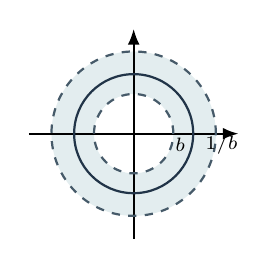
\begin{tikzpicture}[scale=0.72]
          \fill[AccentColor, fill opacity=0.18, even odd rule] (0,0) circle (1.45) (0,0) circle (0.7);
          \draw[-{Latex[length=2mm]}, thick] (-1.85,0) -- (1.85,0);
          \draw[-{Latex[length=2mm]}, thick] (0,-1.85) -- (0,1.85);
          \draw[dashed, thick, DarkGray] (0,0) circle (0.7);
          \draw[dashed, thick, DarkGray] (0,0) circle (1.45);
          \draw[thick, PrimaryColor] (0,0) circle (1.05);
          \node at (0.82,-0.2) {\scriptsize $b$};
          \node at (1.55,-0.2) {\scriptsize $1/b$};
        \end{tikzpicture}
      \end{center}
    \end{column}
  \end{columns}
\end{frame}

\begin{frame}[t]{Properties 7--9}
  \footnotesize
  \begin{conceptbox}{Property 7}
    If $X(z)$ is rational, the ROC is bounded by poles or extends all the way to $0$ and/or $\infty$.
  \end{conceptbox}

  \begin{columns}[T]
    \begin{column}{0.5\textwidth}
      \begin{conceptbox}{Property 8}
        If $X(z)$ is rational and $x[n]$ is right-sided, the ROC is outside the outermost pole.
      \end{conceptbox}
      More precisely: the ROC is outside the circle through the finite pole of largest magnitude.
      If the sequence is causal, the ROC also includes $z=\infty$.
    \end{column}
    \begin{column}{0.5\textwidth}
      \begin{conceptbox}{Property 9}
        If $X(z)$ is rational and $x[n]$ is left-sided, the ROC is inside the innermost \textbf{nonzero} pole.
      \end{conceptbox}
      More precisely: it extends inward and may include $z=0$.
      If the sequence is anticausal, the ROC includes $z=0$.
    \end{column}
  \end{columns}

  \vspace{0.08cm}
  \begin{insightbox}{Same Algebra / Different Signals}
    Poles draw the possible circular boundaries. The ROC chooses the side:
    exterior $\Rightarrow$ right-sided, interior $\Rightarrow$ left-sided, annulus $\Rightarrow$ two-sided.
  \end{insightbox}
\end{frame}

\begin{frame}[t]{Example 10.8: Three Possible ROCs}
  \small
  \begin{columns}[T]
    \begin{column}{0.54\textwidth}
      Consider
      \[
        X(z)=\frac{1}{\left(1-\frac12 z^{-1}\right)\left(1-2z^{-1}\right)}.
      \]
      The poles are at
      \[
        z=\frac12,\qquad z=2.
      \]
      Hence there are three possible ROCs:
      \[
        |z|>2,\qquad \frac12<|z|<2,\qquad |z|<\frac12.
      \]

      \begin{itemize}
        \item Exterior ROC: right-sided sequence.
        \item Interior ROC: left-sided sequence.
        \item Middle annulus: two-sided sequence.
        \item Only the middle annulus includes the unit circle, so only that one has a DTFT.
      \end{itemize}
    \end{column}
    \begin{column}{0.46\textwidth}
      \begin{center}
        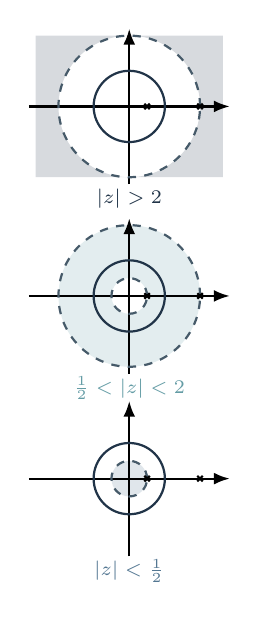
\begin{tikzpicture}[scale=0.58]
          \begin{scope}[yshift=3.15cm]
            \fill[PrimaryColor, fill opacity=0.18, even odd rule] (-2.05,-1.55) rectangle (2.05,1.55) (0,0) circle (1.55);
            \draw[-{Latex[length=2mm]}, thick] (-2.2,0) -- (2.2,0);
            \draw[-{Latex[length=2mm]}, thick] (0,-1.7) -- (0,1.7);
            \draw[thick, PrimaryColor] (0,0) circle (0.78);
            \draw[dashed, thick, DarkGray] (0,0) circle (1.55);
            \draw[thick] (0.33,0.06) -- (0.45,-0.06);
            \draw[thick] (0.33,-0.06) -- (0.45,0.06);
            \draw[thick] (1.49,0.06) -- (1.61,-0.06);
            \draw[thick] (1.49,-0.06) -- (1.61,0.06);
            \node[PrimaryColor] at (0,-2.02) {\scriptsize $|z|>2$};
          \end{scope}
          \begin{scope}[yshift=-1cm]
            \fill[AccentColor, fill opacity=0.18, even odd rule] (0,0) circle (1.55) (0,0) circle (0.39);
            \draw[-{Latex[length=2mm]}, thick] (-2.2,0) -- (2.2,0);
            \draw[-{Latex[length=2mm]}, thick] (0,-1.7) -- (0,1.7);
            \draw[thick, PrimaryColor] (0,0) circle (0.78);
            \draw[dashed, thick, DarkGray] (0,0) circle (0.39);
            \draw[dashed, thick, DarkGray] (0,0) circle (1.55);
            \draw[thick] (0.33,0.06) -- (0.45,-0.06);
            \draw[thick] (0.33,-0.06) -- (0.45,0.06);
            \draw[thick] (1.49,0.06) -- (1.61,-0.06);
            \draw[thick] (1.49,-0.06) -- (1.61,0.06);
            \node[AccentColor] at (0,-2.02) {\scriptsize $\frac12<|z|<2$};
          \end{scope}
          \begin{scope}[yshift=-5cm]
            \fill[SecondaryColor, fill opacity=0.18] (0,0) circle (0.39);
            \draw[-{Latex[length=2mm]}, thick] (-2.2,0) -- (2.2,0);
            \draw[-{Latex[length=2mm]}, thick] (0,-1.7) -- (0,1.7);
            \draw[thick, PrimaryColor] (0,0) circle (0.78);
            \draw[dashed, thick, DarkGray] (0,0) circle (0.39);
            \draw[thick] (0.33,0.06) -- (0.45,-0.06);
            \draw[thick] (0.33,-0.06) -- (0.45,0.06);
            \draw[thick] (1.49,0.06) -- (1.61,-0.06);
            \draw[thick] (1.49,-0.06) -- (1.61,0.06);
            \node[SecondaryColor] at (0,-2.02) {\scriptsize $|z|<\frac12$};
          \end{scope}
        \end{tikzpicture}
      \end{center}
    \end{column}
  \end{columns}
\end{frame}

\section{The Inverse z-Transform}

\begin{frame}[t]{The Inverse z-Transform}
  \small
  Recall
  \[
    X(re^{j\omega})=\mathcal{F}\{x[n]r^{-n}\}.
  \]
  If the circle $|z|=r$ lies in the ROC, apply the inverse DTFT:
  \[
    x[n]r^{-n}
    = \frac{1}{2\pi}\int_{2\pi} X(re^{j\omega})e^{j\omega n}d\omega.
  \]
  Multiply by $r^n$:
  \[
    x[n]
    = \frac{1}{2\pi}\int_{2\pi} X(re^{j\omega})(re^{j\omega})^n d\omega.
  \]
  With $z=re^{j\omega}$ and $dz=jre^{j\omega}d\omega = jz\,d\omega$, we obtain
  \[
    x[n]
    = \frac{1}{2\pi j}\oint_C X(z)z^{n-1}\,dz
  \]
  where $C$ is any counterclockwise closed contour lying entirely within the ROC.

  \vspace{0.1cm}
  \begin{conceptbox}{Inverse z-Transform}
    \[
      x[n] = \frac{1}{2\pi j}\oint_C X(z)z^{n-1}\,dz
    \]
  \end{conceptbox}

\end{frame}

\begin{frame}[t]{Example 10.9: Partial Fractions with an Exterior ROC}
  \small
  \begin{columns}[T]
    \begin{column}{0.56\textwidth}
      Consider
      \[
        X(z)=\frac{3-\frac52 z^{-1}}
        {\left(1-\frac14 z^{-1}\right)\left(1-\frac13 z^{-1}\right)},
        \qquad |z|>\frac13.
      \]
      Partial fractions give
      \[
        X(z)=\frac{1}{1-\frac14 z^{-1}} + \frac{2}{1-\frac13 z^{-1}}.
      \]
      Because the ROC is outside the outermost pole, \textit{both} terms are right-sided:
      \[
        \frac{1}{1-\frac14 z^{-1}}
        \stackrel{\mathcal{Z}}{\longleftrightarrow}
        \left(\frac14\right)^n u[n],
      \]
      \[
        \frac{2}{1-\frac13 z^{-1}}
        \stackrel{\mathcal{Z}}{\longleftrightarrow}
        2\left(\frac13\right)^n u[n].
      \]
      Hence
      \[
        x[n]=\left(\frac14\right)^n u[n]
        + 2\left(\frac13\right)^n u[n].
      \]
    \end{column}
    \begin{column}{0.44\textwidth}
      \begin{center}
        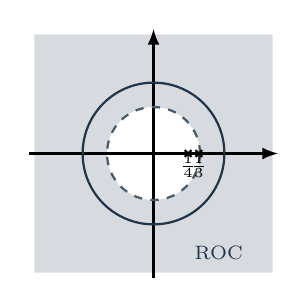
\begin{tikzpicture}[scale=0.72]
          \fill[PrimaryColor, fill opacity=0.18, even odd rule] (-2.1,-2.1) rectangle (2.1,2.1) (0,0) circle (0.82);
          \draw[-{Latex[length=2mm]}, thick] (-2.2,0) -- (2.2,0);
          \draw[-{Latex[length=2mm]}, thick] (0,-2.2) -- (0,2.2);
          \draw[thick, PrimaryColor] (0,0) circle (1.25);
          \draw[dashed, thick, DarkGray] (0,0) circle (0.82);
          \draw[thick] (0.55,0.06) -- (0.67,-0.06);
          \draw[thick] (0.55,-0.06) -- (0.67,0.06);
          \draw[thick] (0.74,0.06) -- (0.86,-0.06);
          \draw[thick] (0.74,-0.06) -- (0.86,0.06);
          \node at (0.61,-0.22) {\scriptsize $\frac14$};
          \node at (0.80,-0.22) {\scriptsize $\frac13$};
          \node[PrimaryColor] at (1.15,-1.75) {\scriptsize ROC};
        \end{tikzpicture}
      \end{center}

      \vspace{0.08cm}
      \begin{insightbox}{Main idea}
        The partial fractions do not change.
        \\
        The \textbf{ROC decides how each term is interpreted}.
      \end{insightbox}
    \end{column}
  \end{columns}
\end{frame}

\begin{frame}[t]{Examples 10.10 and 10.11: The Same Algebraic \texorpdfstring{$X(z)$}{X(z)} Gives Different Sequences}
  \small
  Keep the same partial-fraction expansion as Example 10.9:
  \[
    X(z)=\frac{1}{1-\frac14 z^{-1}} + \frac{2}{1-\frac13 z^{-1}}.
  \]
  \begin{columns}[T]
    \begin{column}{0.5\textwidth}
      \textbf{Example 10.10}\\
      ROC:
      \[
        \frac14<|z|<\frac13.
      \]
      Then the first term is right-sided but the second is left-sided:
      \[
        x[n]
        =
        \left(\frac14\right)^n u[n]
        -
        2\left(\frac13\right)^n u[-n-1].
      \]
      \begin{center}
        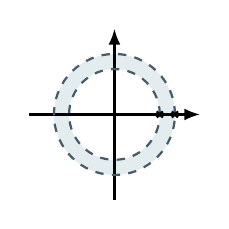
\begin{tikzpicture}[scale=0.64]
          \fill[AccentColor, fill opacity=0.18, even odd rule] (0,0) circle (1.2) (0,0) circle (0.9);
          \draw[-{Latex[length=2mm]}, thick] (-1.7,0) -- (1.7,0);
          \draw[-{Latex[length=2mm]}, thick] (0,-1.7) -- (0,1.7);
          \draw[dashed, thick, DarkGray] (0,0) circle (0.9);
          \draw[dashed, thick, DarkGray] (0,0) circle (1.2);
          \draw[thick] (0.84,0.06) -- (0.96,-0.06);
          \draw[thick] (0.84,-0.06) -- (0.96,0.06);
          \draw[thick] (1.14,0.06) -- (1.26,-0.06);
          \draw[thick] (1.14,-0.06) -- (1.26,0.06);
        \end{tikzpicture}
      \end{center}
    \end{column}
    \begin{column}{0.5\textwidth}
      \textbf{Example 10.11}\\
      ROC:
      \[
        |z|<\frac14.
      \]
      Now both terms are left-sided:
      \[
        x[n]
        =
        -
        \left(\frac14\right)^n u[-n-1]
        -
        2\left(\frac13\right)^n u[-n-1].
      \]
      \begin{center}
        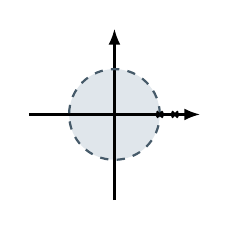
\begin{tikzpicture}[scale=0.64]
          \fill[SecondaryColor, fill opacity=0.18] (0,0) circle (0.9);
          \draw[-{Latex[length=2mm]}, thick] (-1.7,0) -- (1.7,0);
          \draw[-{Latex[length=2mm]}, thick] (0,-1.7) -- (0,1.7);
          \draw[dashed, thick, DarkGray] (0,0) circle (0.9);
          \draw[thick] (0.84,0.06) -- (0.96,-0.06);
          \draw[thick] (0.84,-0.06) -- (0.96,0.06);
          \draw[thick] (1.14,0.06) -- (1.26,-0.06);
          \draw[thick] (1.14,-0.06) -- (1.26,0.06);
        \end{tikzpicture}
      \end{center}
    \end{column}
  \end{columns}
\end{frame}

\begin{frame}[t]{Power-Series Inversion: Examples 10.12 and 10.13}
  \scriptsize
  \begin{insightbox}{Intuition}
    Rewrite $X(z)$ as a power series that is valid in the ROC, then match it with
    \[
      X(z)=\sum_{n=-\infty}^{\infty}x[n]z^{-n}.
    \]
    The coefficient of $z^{-n}$ is $x[n]$; positive powers of $z$ therefore represent negative-time samples.
  \end{insightbox}

  \vspace{-0.12cm}
  \begin{itemize}
    \setlength{\itemsep}{0.08em}
    \item \textbf{Example 10.12}
      \[
        X(z)=4z^2+2+3z^{-1}
        \quad\Longrightarrow\quad
        x[n]=4\delta[n+2]+2\delta[n]+3\delta[n-1].
      \]

    \item \textbf{Example 10.13}
      \[
        X(z)=\frac{1}{1-az^{-1}}.
      \]
      If $|z|>|a|$ $(|az^{-1}|<1)$,
      \[
        X(z)=1+az^{-1}+a^2z^{-2}+\cdots
        \quad\Longrightarrow\quad
        x[n]=a^n u[n].
      \]
      If $|z|<|a|$ $(|z/a|<1)$,
      \[
        X(z)=-\frac{z/a}{1-z/a}
        =-a^{-1}z-a^{-2}z^2-a^{-3}z^3-\cdots
        \quad\Longrightarrow\quad
        x[n]=-a^n u[-n-1].
      \]

  \end{itemize}
\end{frame}

\begin{frame}[t]{Power-Series Inversion: Example 10.14}
  \small
  Consider
  \[
    X(z)=\log(1+az^{-1}), \qquad |z|>|a|.
  \]
  Using the Taylor series
  \[
    \log(1+v)=\sum_{n=1}^{\infty}\frac{(-1)^{n+1}v^n}{n},
    \qquad |v|<1,
  \]
  with $v=az^{-1}$, we obtain
  \[
    X(z)=\sum_{n=1}^{\infty}\frac{(-1)^{n+1}a^n z^{-n}}{n}.
  \]
  Matching powers of $z^{-n}$ gives
  \[
    x[n]=
    \begin{cases}
      (-1)^{n+1}\dfrac{a^n}{n}, & n\ge 1 \\
      0, & n\le 0.
    \end{cases}
  \]
  \begin{insightbox}{Why power series help}
    The coefficient of $z^{-n}$ in the expansion is exactly the sequence value $x[n]$.
  \end{insightbox}
\end{frame}

\section{Properties of the z-Transform}

\begin{frame}[t]{Linearity and Time Shifting}
  \small
  \begin{columns}[T]
    \begin{column}{0.52\textwidth}
      \begin{conceptbox}{Linearity}
        If
        \[
          x_1[n]\stackrel{\mathcal{Z}}{\longleftrightarrow}X_1(z), \qquad
          x_2[n]\stackrel{\mathcal{Z}}{\longleftrightarrow}X_2(z),
        \]
        then
        \[
          ax_1[n]+bx_2[n]
          \stackrel{\mathcal{Z}}{\longleftrightarrow}
          aX_1(z)+bX_2(z)
        \]
        with ROC containing at least $R_1\cap R_2$.
      \end{conceptbox}

      \textit{Justification:}
      the defining sum is linear. The ROC is at least the intersection;
      it can be larger if pole-zero cancellation occurs.

      \vspace{0.08cm}
      \textbf{Example}
      \[
        7\left(\frac13\right)^n u[n]-6\left(\frac12\right)^n u[n]
      \]
      is Example 10.3.
    \end{column}
    \begin{column}{0.48\textwidth}
      \begin{conceptbox}{Time Shifting}
        If
        \[
          x[n]\stackrel{\mathcal{Z}}{\longleftrightarrow}X(z),
        \]
        then
        \[
          x[n-n_0]
          \stackrel{\mathcal{Z}}{\longleftrightarrow}
          z^{-n_0}X(z)
        \]
        with the same ROC, except possibly for adding or deleting $0$ or $\infty$.
      \end{conceptbox}

      \textit{Proof sketch:}
      \[
        \sum_{n=-\infty}^{\infty} x[n-n_0]z^{-n}
        = z^{-n_0}\sum_{m=-\infty}^{\infty}x[m]z^{-m}.
      \]
      The multiplier $z^{-n_0}$ can add/delete a pole at $0$ or at $\infty$,
      but it does not move any finite nonzero boundary.

      \vspace{0.08cm}
      \textbf{Example}
      \[
        \delta[n-1]
        \stackrel{\mathcal{Z}}{\longleftrightarrow}
        z^{-1}.
      \]
    \end{column}
  \end{columns}
\end{frame}

\begin{frame}[t]{Scaling, Time Reversal, and Conjugation}
  \scriptsize
  \begin{columns}[T]
    \begin{column}{0.55\textwidth}
      \begin{conceptbox}{Scaling in the z-domain}
        \[
          a_0^n x[n]
          \stackrel{\mathcal{Z}}{\longleftrightarrow}
          X\!\left(\frac{z}{a_0}\right)
        \]
        and the ROC scales by $|a_0|$.
      \end{conceptbox}
      \textit{Proof:}
      \[
        \sum a_0^n x[n]z^{-n}
        = \sum x[n]\left(\frac{z}{a_0}\right)^{-n}.
      \]
      Multiplying by $e^{j\omega_0 n}$ rotates the pole-zero pattern; multiplying by $r_0^n$ scales its radii.

      \vspace{0.08cm}
      \begin{conceptbox}{Time Reversal}
        \[
          x[-n]
          \stackrel{\mathcal{Z}}{\longleftrightarrow}
          X(z^{-1})
        \]
        with inverted ROC.
      \end{conceptbox}
      \textit{Proof:}
      \[
        \sum x[-n]z^{-n}
        =\sum_m x[m](z^{-1})^{-m}.
      \]
    \end{column}
    \begin{column}{0.45\textwidth}
      \begin{center}
        \textbf{Effect of multiplying by $e^{j\omega_0 n}$}\\[0.05cm]
        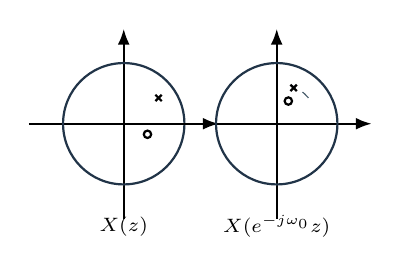
\begin{tikzpicture}[scale=0.67]
          \begin{scope}[xshift=-1.45cm]
            \draw[-{Latex[length=2mm]}, thick] (-1.8,0) -- (1.8,0);
            \draw[-{Latex[length=2mm]}, thick] (0,-1.8) -- (0,1.8);
            \draw[thick, PrimaryColor] (0,0) circle (1.15);
            \draw[thick] (0.6,0.55) -- (0.72,0.43);
            \draw[thick] (0.6,0.43) -- (0.72,0.55);
            \draw[thick] (0.45,-0.2) circle (0.07);
            \node at (0,-1.95) {\scriptsize $X(z)$};
          \end{scope}
          \begin{scope}[xshift=1.45cm]
            \draw[-{Latex[length=2mm]}, thick] (-1.8,0) -- (1.8,0);
            \draw[-{Latex[length=2mm]}, thick] (0,-1.8) -- (0,1.8);
            \draw[thick, PrimaryColor] (0,0) circle (1.15);
            \draw[dashed, DarkGray] (0.6,0.49) arc[start angle=39,end angle=69,radius=0.78];
            \draw[thick] (0.26,0.74) -- (0.38,0.62);
            \draw[thick] (0.26,0.62) -- (0.38,0.74);
            \draw[thick] (0.22,0.43) circle (0.07);
            \node at (0,-1.95) {\scriptsize $X(e^{-j\omega_0}z)$};
          \end{scope}
        \end{tikzpicture}
      \end{center}

      \vspace{0.06cm}
      \begin{conceptbox}{Conjugation}
        \[
          x^*[n]
          \stackrel{\mathcal{Z}}{\longleftrightarrow}
          X^*(z^*)
        \]
        with the same ROC.
      \end{conceptbox}
      {\tiny
        \[
          \sum x^*[n]z^{-n}
          =\left(\sum x[n](z^*)^{-n}\right)^*
          =X^*(z^*).
        \]
      For real $x[n]$, $X(z)=X^*(z^*)$, so nonreal poles and zeros occur in conjugate pairs and the ROC is symmetric about the real axis.}
    \end{column}
  \end{columns}
\end{frame}

\begin{frame}[t]{Time Expansion}
  \small
  Define the expanded sequence
  \[
    x_{(k)}[n]=
    \begin{cases}
      x[n/k], & n \text{ is an integer multiple of } k,\\
      0, & n \text{ is not a multiple of } k.
    \end{cases}
  \]

  \begin{columns}[T]
    \begin{column}{0.5\textwidth}
      \begin{conceptbox}{Time expansion property}
        \[
          x_{(k)}[n]
          \stackrel{\mathcal{Z}}{\longleftrightarrow}
          X(z^k),
        \]
        with ROC $R^{1/k}$.
      \end{conceptbox}

      \textit{Proof from the series:}
      \[
        \sum_{n=-\infty}^{\infty}x_{(k)}[n]z^{-n}
        =
        \sum_{m=-\infty}^{\infty}x[m]z^{-km}
        =
        X(z^k).
      \]
    \end{column}
    \begin{column}{0.5\textwidth}
      \begin{center}
        \textbf{Insert $k-1$ zeros between samples}\\[-0.02cm]
        \begin{tikzpicture}
          \begin{axis}[
              width=0.9\textwidth, height=2.2cm,
              axis lines=middle, axis line style={-{Latex[length=2mm]}},
              xmin=-0.5, xmax=5.5, ymin=-0.1, ymax=1.2,
              xtick={0,1,2,3,4,5}, ytick=\empty,
              clip=false
            ]
            \addplot+[discrete] coordinates {(0,0.35) (1,1) (2,0.7) (3,0.25)};
          \end{axis}
        \end{tikzpicture}

        \vspace{0.06cm}
        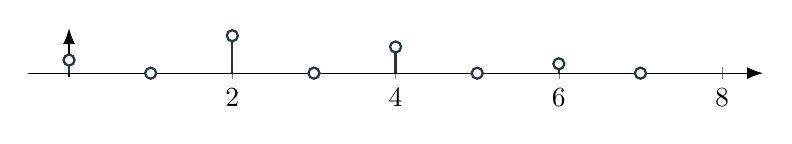
\begin{tikzpicture}
          \begin{axis}[
              width=0.9\textwidth, height=2.2cm,
              axis lines=middle, axis line style={-{Latex[length=2mm]}},
              xmin=-0.5, xmax=8.5, ymin=-0.1, ymax=1.2,
              xtick={0,2,4,6,8}, ytick=\empty,
              clip=false
            ]
            \addplot+[discrete] coordinates {(0,0.35) (1,0) (2,1) (3,0) (4,0.7) (5,0) (6,0.25) (7,0)};
          \end{axis}
        \end{tikzpicture}
      \end{center}

      \begin{insightbox}{ROC Geometry}
        $z$ is in the new ROC exactly when $z^k$ is in the old ROC,
        so radii are mapped by $r\mapsto r^k$.
      \end{insightbox}
    \end{column}
  \end{columns}
\end{frame}

\begin{frame}[t]{Convolution Property and Proof}
  \scriptsize
  \begin{conceptbox}{Convolution}
    \[
      y[n]=x_1[n]*x_2[n]
      \stackrel{\mathcal{Z}}{\longleftrightarrow}
      Y(z)=X_1(z)X_2(z)
    \]
    with ROC containing at least $R_1\cap R_2$; cancellation may enlarge it.
  \end{conceptbox}

  Starting from
  \[
    y[n]=\sum_{k=-\infty}^{\infty}x_1[k]x_2[n-k],
  \]
  we obtain
  \[
    \begin{aligned}
      Y(z)
      &=\sum_{n=-\infty}^{\infty}
      \sum_{k=-\infty}^{\infty}
      x_1[k]x_2[n-k]z^{-n}\\
      &=\sum_{k=-\infty}^{\infty}x_1[k]z^{-k}
      \sum_{m=-\infty}^{\infty}x_2[m]z^{-m}
      \qquad (m=n-k)\\
      &=X_1(z)X_2(z).
    \end{aligned}
  \]

  \begin{insightbox}{ROC Nuance}
    Convergence is guaranteed wherever both series converge, so the ROC includes
    at least $R_1\cap R_2$. If a pole is cancelled in the product, the final ROC can be larger.
  \end{insightbox}
\end{frame}

\begin{frame}[t]{First Difference and Accumulation}
  \footnotesize
  \begin{columns}[T]
    \begin{column}{0.50\textwidth}
      \begin{conceptbox}{First Difference: Example 10.15}
        For $h[n]=\delta[n]-\delta[n-1]$,
        \[
          y[n]=x[n]-x[n-1]
          \stackrel{\mathcal{Z}}{\longleftrightarrow}
          (1-z^{-1})X(z),
        \]
        with ROC at least $R$ except possible deletion of $z=0$; cancellation may add $z=1$.
      \end{conceptbox}
      First difference is the discrete-time counterpart of differentiation.
    \end{column}
    \begin{column}{0.50\textwidth}
      \begin{conceptbox}{Accumulation}
        Example 10.16 defines the running sum
        \[
          w[n]=\sum_{k=-\infty}^{n}x[k].
        \]
        Since
        \[
          w[n]=u[n]*x[n],
        \]
        and
        \[
          u[n]
          \stackrel{\mathcal{Z}}{\longleftrightarrow}
          \frac{1}{1-z^{-1}},
          \qquad |z|>1,
        \]
        we get
        \[
          W(z)=\frac{1}{1-z^{-1}}X(z).
        \]
        ROC contains at least $R\cap\{|z|>1\}$.
      \end{conceptbox}
      \textit{Intuition:}
      convolution with $u[n]$ is the discrete-time counterpart of integration.
    \end{column}
  \end{columns}
\end{frame}

\begin{frame}[t]{Differentiation in the z-Domain}
  \footnotesize
  \begin{conceptbox}{Differentiation in the z-domain}
    \[
      n\,x[n]
      \stackrel{\mathcal{Z}}{\longleftrightarrow}
      -z\frac{dX(z)}{dz}
    \]
    with ROC $=R$.
  \end{conceptbox}

  \textit{Proof:}
  \[
    \frac{dX}{dz}
    =\sum_n (-n)x[n]z^{-n-1};
    \qquad -z\frac{dX}{dz}=\sum_n n x[n]z^{-n}.
  \]

  \textbf{Example 10.18}
  Starting from
  \[
    a^n u[n]
    \stackrel{\mathcal{Z}}{\longleftrightarrow}
    \frac{1}{1-az^{-1}},
  \]
  differentiation gives
  \[
    n a^n u[n]
    \stackrel{\mathcal{Z}}{\longleftrightarrow}
    \frac{az^{-1}}{(1-az^{-1})^2}.
  \]
\end{frame}

\begin{frame}[t]{Difference Equations as a z-Transform Property}
  \small
  \begin{conceptbox}{Linear constant-coefficient difference equation}
    If
    \[
      \sum_{k=0}^{N} a_k\,y[n-k]
      =
      \sum_{k=0}^{M} b_k\,x[n-k],
    \]
    then, using linearity and time shifting,
    \[
      H(z)=\frac{Y(z)}{X(z)}
      =
      \frac{\sum_{k=0}^{M} b_k z^{-k}}
      {\sum_{k=0}^{N} a_k z^{-k}}.
    \]
  \end{conceptbox}

  \begin{columns}[T]
    \begin{column}{0.52\textwidth}
      \textit{Justification:}
      \[
        \mathcal{Z}\{y[n-k]\}=z^{-k}Y(z),
        \qquad
        \mathcal{Z}\{x[n-k]\}=z^{-k}X(z).
      \]
      Then factor $Y(z)$ on the left and $X(z)$ on the right.
    \end{column}
    \begin{column}{0.48\textwidth}
      \begin{insightbox}{Book warning}
        The difference equation determines the \textbf{algebraic} system function,
        but not the ROC. The ROC is extra information: it decides causality,
        stability, and the impulse response.
      \end{insightbox}
    \end{column}
  \end{columns}
\end{frame}

\begin{frame}[t]{Summary of z-Transform Properties}
  \scriptsize
  \centering
  \begingroup
  \setlength{\tabcolsep}{3pt}
  \renewcommand{\arraystretch}{1.28}
  \begin{tabular}{>{\raggedright\arraybackslash}p{0.23\textwidth}
      >{\raggedright\arraybackslash}p{0.25\textwidth}
      >{\raggedright\arraybackslash}p{0.28\textwidth}
    >{\raggedright\arraybackslash}p{0.16\textwidth}}
    \toprule
    Property & Time-domain signal & z-domain expression & ROC / nuance \\
    \midrule
    Linearity
    & $a x_1[n]+b x_2[n]$
    & $aX_1(z)+bX_2(z)$
    & $\supseteq R_1\cap R_2$ \\
    Time shift
    & $x[n-n_0]$
    & $z^{-n_0}X(z)$
    & same $R$, except $0,\infty$ \\
    Scaling
    & $a_0^n x[n]$
    & $X(z/a_0)$
    & $|a_0|R$ \\
    Time reversal
    & $x[-n]$
    & $X(z^{-1})$
    & inverted $R$ \\
    Conjugation
    & $x^*[n]$
    & $X^*(z^*)$
    & same $R$ \\
    Time expansion
    & $x_{(k)}[n]$: insert $k-1$ zeros
    & $X(z^k)$
    & $R^{1/k}$ \\
    Convolution
    & $x_1[n]*x_2[n]$
    & $X_1(z)X_2(z)$
    & $\supseteq R_1\cap R_2$ \\
    First difference
    & $x[n]-x[n-1]$
    & $(1-z^{-1})X(z)$
    & possible $0$ deletion, $1$ cancellation \\
    Accumulation
    & $\sum_{k=-\infty}^{n}x[k]$
    & $\frac{1}{1-z^{-1}}X(z)$
    & $\supseteq R\cap\{|z|>1\}$ \\
    z-domain differentiation
    & $n x[n]$
    & $-z\,dX(z)/dz$
    & same $R$ \\
    Initial value
    & causal/right-sided from $0$
    & $x[0]=\lim_{z\to\infty}X(z)$
    & requires $x[n]=0,\ n<0$ \\
    LCCDE
    & $\sum a_k y[n-k]=\sum b_k x[n-k]$
    & $H(z)=\frac{\sum b_k z^{-k}}{\sum a_k z^{-k}}$
    & equation alone does not set ROC \\
    \bottomrule
  \end{tabular}
  \endgroup
\end{frame}

\section{Analysis of LTI Systems}

\begin{frame}[t]{Transform-Domain View of an LTI System}
  \small
  \begin{columns}[T]
    \begin{column}{0.55\textwidth}
      \begin{itemize}
        \item For an LTI system with impulse response $h[n]$,
          \[
            Y(z)=H(z)X(z).
          \]
        \item The z-transform converts convolution into multiplication.
        \item If the ROC of $H(z)$ includes the unit circle, then
          \[
            H(e^{j\omega})
          \]
          is the \textbf{frequency response}.
        \item So poles, zeros, and the ROC describe not only the algebra of the transform, but also the behavior of the system.
      \end{itemize}
      \begin{insightbox}{Main payoff}
        Just as with Laplace transforms, many system properties become visible directly in the transform domain.
      \end{insightbox}
    \end{column}
    \begin{column}{0.45\textwidth}
      \begin{center}
        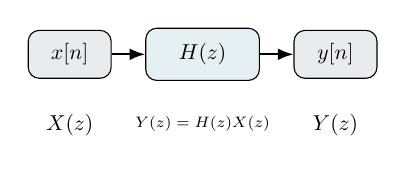
\begin{tikzpicture}[node distance=0.45cm, scale=0.78, transform shape]
          \node[draw, rounded corners, fill=PrimaryColor!10, minimum width=1.35cm, minimum height=0.78cm] (x) {$x[n]$};
          \node[draw, rounded corners, fill=AccentColor!16, minimum width=1.85cm, minimum height=0.85cm, right=0.55cm of x] (h) {$H(z)$};
          \node[draw, rounded corners, fill=PrimaryColor!10, minimum width=1.35cm, minimum height=0.78cm, right=0.55cm of h] (y) {$y[n]$};
          \draw[-{Latex[length=2mm]}, thick] (x) -- (h);
          \draw[-{Latex[length=2mm]}, thick] (h) -- (y);

          \node[below=0.45cm of x] {$X(z)$};
          \node[below=0.45cm of h] {\scriptsize $Y(z)=H(z)X(z)$};
          \node[below=0.45cm of y] {$Y(z)$};
        \end{tikzpicture}
      \end{center}

      \vspace{0.15cm}
      \begin{conceptbox}{Eigenfunction Reminder}
        For input $x[n]=z^n$,
        \[
          y[n]=H(z)z^n.
        \]
      \end{conceptbox}
    \end{column}
  \end{columns}
\end{frame}

\begin{frame}[t]{Causality from the ROC: Examples 10.20 and 10.21}
  \small
  \begin{columns}[T]
    \begin{column}{0.57\textwidth}
      \begin{conceptbox}{Causality Test}
        A discrete-time LTI system is causal iff the ROC of $H(z)$ is the exterior of a circle and includes $\infty$.
      \end{conceptbox}

      \textbf{Example 10.20}
      \[
        H(z)=\frac{z^3-2z^2+z}{z^2+\frac14 z+\frac18}
      \]
      is \textbf{not causal} because the numerator degree exceeds the denominator degree when written in powers of $z$.

      \vspace{0.08cm}
      \textbf{Example 10.21}
      \[
        H(z)=\frac{1}{1-\frac12 z^{-1}}+\frac{1}{1-2z^{-1}},
        \qquad |z|>2.
      \]
      The ROC is outside the outermost pole and includes $\infty$, so the system is causal.
    \end{column}
    \begin{column}{0.43\textwidth}
      \begin{center}
        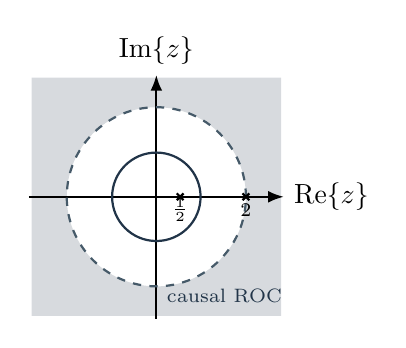
\begin{tikzpicture}[scale=0.72]
          \fill[PrimaryColor, fill opacity=0.18, even odd rule] (-2.2,-2.1) rectangle (2.2,2.1) (0,0) circle (1.58);
          \draw[-{Latex[length=2mm]}, thick] (-2.25,0) -- (2.25,0) node[right] {$\text{Re}\{z\}$};
          \draw[-{Latex[length=2mm]}, thick] (0,-2.15) -- (0,2.15) node[above] {$\text{Im}\{z\}$};
          \draw[thick, PrimaryColor] (0,0) circle (0.78);
          \draw[dashed, thick, DarkGray] (0,0) circle (1.58);
          \draw[thick] (0.36,0.06) -- (0.48,-0.06);
          \draw[thick] (0.36,-0.06) -- (0.48,0.06);
          \draw[thick] (1.52,0.06) -- (1.64,-0.06);
          \draw[thick] (1.52,-0.06) -- (1.64,0.06);
          \node at (0.42,-0.23) {\scriptsize $\frac12$};
          \node at (1.58,-0.23) {\scriptsize $2$};
          \node[PrimaryColor] at (1.2,-1.75) {\scriptsize causal ROC};
        \end{tikzpicture}
      \end{center}
    \end{column}
  \end{columns}
\end{frame}

\begin{frame}[t]{Stability from the ROC: Examples 10.22--10.24}
  \footnotesize
  \begin{columns}[T]
    \begin{column}{0.54\textwidth}
      \begin{conceptbox}{Stability Test}
        An LTI system is stable iff the ROC of $H(z)$ includes the unit circle.
      \end{conceptbox}

      \begin{itemize}
        \item \textbf{Example 10.22:}
          the same algebraic $H(z)$ from Example 10.21 is unstable if the ROC is $|z|<2$.
        \item \textbf{Example 10.23:}
          for the causal first-order system
          \[
            H(z)=\frac{1}{1-az^{-1}},
          \]
          stability requires $|a|<1$.
        \item \textbf{Example 10.24:}
          if
          \[
            H(z)=\frac{1}{1-2r\cos\theta\, z^{-1}+r^2 z^{-2}},
          \]
          then the poles are at $re^{\pm j\theta}$, so a causal system is stable iff $r<1$.
      \end{itemize}
    \end{column}
    \begin{column}{0.46\textwidth}
      \begin{center}
        \textbf{Complex poles and the unit circle}\\[0.05cm]
        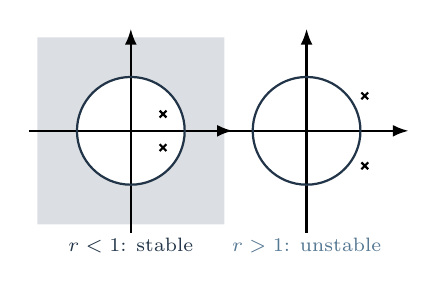
\begin{tikzpicture}[scale=0.72]
          \begin{scope}[xshift=-1.55cm]
            \fill[PrimaryColor, fill opacity=0.16, even odd rule] (-1.65,-1.65) rectangle (1.65,1.65) (0,0) circle (0.95);
            \draw[-{Latex[length=2mm]}, thick] (-1.8,0) -- (1.8,0);
            \draw[-{Latex[length=2mm]}, thick] (0,-1.8) -- (0,1.8);
            \draw[thick, PrimaryColor] (0,0) circle (0.95);
            \draw[thick] (35:0.62) -- ++(0.12,-0.12);
            \draw[thick] (35:0.62) ++(0,-0.12) -- ++(0.12,0.12);
            \draw[thick] (-35:0.62) -- ++(0.12,0.12);
            \draw[thick] (-35:0.62) ++(0,0.12) -- ++(0.12,-0.12);
            \node[PrimaryColor] at (0,-2.02) {\scriptsize $r<1$: stable};
          \end{scope}
          \begin{scope}[xshift=1.55cm]
            \draw[-{Latex[length=2mm]}, thick] (-1.8,0) -- (1.8,0);
            \draw[-{Latex[length=2mm]}, thick] (0,-1.8) -- (0,1.8);
            \draw[thick, PrimaryColor] (0,0) circle (0.95);
            \draw[thick] (35:1.18) -- ++(0.12,-0.12);
            \draw[thick] (35:1.18) ++(0,-0.12) -- ++(0.12,0.12);
            \draw[thick] (-35:1.18) -- ++(0.12,0.12);
            \draw[thick] (-35:1.18) ++(0,0.12) -- ++(0.12,-0.12);
            \node[SecondaryColor] at (0,-2.02) {\scriptsize $r>1$: unstable};
          \end{scope}
        \end{tikzpicture}
      \end{center}
    \end{column}
  \end{columns}
\end{frame}

\begin{frame}[t]{Example 10.25: Difference Equations Become Algebra}
  \small
  Consider the linear constant-coefficient difference equation
  \[
    y[n]-\frac12 y[n-1] = x[n]+\frac13 x[n-1].
  \]
  Taking z-transforms and using linearity and time shifting,
  \[
    Y(z)-\frac12 z^{-1}Y(z)=X(z)+\frac13 z^{-1}X(z).
  \]
  So
  \[
    Y(z)=X(z)\frac{1+\frac13 z^{-1}}{1-\frac12 z^{-1}}
  \]
  and therefore
  \[
    H(z)\triangleq \frac{Y(z)}{X(z)}
    =
    \frac{1+\frac13 z^{-1}}{1-\frac12 z^{-1}}.
  \]

  The difference equation fixes the algebraic form of $H(z)$, but not the ROC:
  \[
    |z|>\frac12 \text{ for the causal interpretation},
    \qquad
    |z|<\frac12 \text{ for the anticausal one}.
  \]

  \vspace{0.08cm}
  Main lesson:
  a difference equation determines the algebraic form of $H(z)$, but the ROC still determines whether the realization is causal, anticausal, or stable.
\end{frame}

\begin{frame}[t]{Solving a Difference Equation by z-Transform}
  \small
  Use the \textbf{causal} system from Example 10.25:
  \[
    H(z)=\frac{1+\frac13 z^{-1}}{1-\frac12 z^{-1}},
    \qquad |z|>\frac12.
  \]
  Let the input be the unit step:
  \[
    x[n]=u[n]
    \stackrel{\mathcal{Z}}{\longleftrightarrow}
    X(z)=\frac{1}{1-z^{-1}},
    \qquad |z|>1.
  \]
  Then
  \[
    Y(z)=H(z)X(z)
    =
    \frac{1+\frac13 z^{-1}}
    {\left(1-\frac12 z^{-1}\right)\left(1-z^{-1}\right)}.
  \]
  Partial fractions give
  \[
    Y(z)=\frac{8/3}{1-z^{-1}}-\frac{5/3}{1-\frac12 z^{-1}}.
  \]
  Hence
  \[
    y[n]=\frac{8}{3}u[n]-\frac{5}{3}\left(\frac12\right)^n u[n].
  \]

  \vspace{0.08cm}
  This is the discrete-time version of what we did with differential equations in the Laplace domain:
  \[
    \text{difference equation} \;\Longrightarrow\; \text{algebra} \;\Longrightarrow\; \text{inverse transform}.
  \]
\end{frame}

\end{document}
